\documentclass[twoside]{book}

% Packages required by doxygen
\usepackage{fixltx2e}
\usepackage{calc}
\usepackage{doxygen}
\usepackage[export]{adjustbox} % also loads graphicx
\usepackage{graphicx}
\usepackage[utf8]{inputenc}
\usepackage{makeidx}
\usepackage{multicol}
\usepackage{multirow}
\PassOptionsToPackage{warn}{textcomp}
\usepackage{textcomp}
\usepackage[nointegrals]{wasysym}
\usepackage[table]{xcolor}

% Font selection
\usepackage[T1]{fontenc}
\usepackage[scaled=.90]{helvet}
\usepackage{courier}
\usepackage{amssymb}
\usepackage{sectsty}
\renewcommand{\familydefault}{\sfdefault}
\allsectionsfont{%
  \fontseries{bc}\selectfont%
  \color{darkgray}%
}
\renewcommand{\DoxyLabelFont}{%
  \fontseries{bc}\selectfont%
  \color{darkgray}%
}
\newcommand{\+}{\discretionary{\mbox{\scriptsize$\hookleftarrow$}}{}{}}

% Page & text layout
\usepackage{geometry}
\geometry{%
  a4paper,%
  top=2.5cm,%
  bottom=2.5cm,%
  left=2.5cm,%
  right=2.5cm%
}
\tolerance=750
\hfuzz=15pt
\hbadness=750
\setlength{\emergencystretch}{15pt}
\setlength{\parindent}{0cm}
\setlength{\parskip}{3ex plus 2ex minus 2ex}
\makeatletter
\renewcommand{\paragraph}{%
  \@startsection{paragraph}{4}{0ex}{-1.0ex}{1.0ex}{%
    \normalfont\normalsize\bfseries\SS@parafont%
  }%
}
\renewcommand{\subparagraph}{%
  \@startsection{subparagraph}{5}{0ex}{-1.0ex}{1.0ex}{%
    \normalfont\normalsize\bfseries\SS@subparafont%
  }%
}
\makeatother

% Headers & footers
\usepackage{fancyhdr}
\pagestyle{fancyplain}
\fancyhead[LE]{\fancyplain{}{\bfseries\thepage}}
\fancyhead[CE]{\fancyplain{}{}}
\fancyhead[RE]{\fancyplain{}{\bfseries\leftmark}}
\fancyhead[LO]{\fancyplain{}{\bfseries\rightmark}}
\fancyhead[CO]{\fancyplain{}{}}
\fancyhead[RO]{\fancyplain{}{\bfseries\thepage}}
\fancyfoot[LE]{\fancyplain{}{}}
\fancyfoot[CE]{\fancyplain{}{}}
\fancyfoot[RE]{\fancyplain{}{\bfseries\scriptsize Generated by Doxygen }}
\fancyfoot[LO]{\fancyplain{}{\bfseries\scriptsize Generated by Doxygen }}
\fancyfoot[CO]{\fancyplain{}{}}
\fancyfoot[RO]{\fancyplain{}{}}
\renewcommand{\footrulewidth}{0.4pt}
\renewcommand{\chaptermark}[1]{%
  \markboth{#1}{}%
}
\renewcommand{\sectionmark}[1]{%
  \markright{\thesection\ #1}%
}

% Indices & bibliography
\usepackage{natbib}
\usepackage[titles]{tocloft}
\setcounter{tocdepth}{3}
\setcounter{secnumdepth}{5}
\makeindex

% Hyperlinks (required, but should be loaded last)
\usepackage{ifpdf}
\ifpdf
  \usepackage[pdftex,pagebackref=true]{hyperref}
\else
  \usepackage[ps2pdf,pagebackref=true]{hyperref}
\fi
\hypersetup{%
  colorlinks=true,%
  linkcolor=blue,%
  citecolor=blue,%
  unicode%
}

% Custom commands
\newcommand{\clearemptydoublepage}{%
  \newpage{\pagestyle{empty}\cleardoublepage}%
}

\usepackage{caption}
\captionsetup{labelsep=space,justification=centering,font={bf},singlelinecheck=off,skip=4pt,position=top}

%===== C O N T E N T S =====

\begin{document}

% Titlepage & ToC
\hypersetup{pageanchor=false,
             bookmarksnumbered=true,
             pdfencoding=unicode
            }
\pagenumbering{alph}
\begin{titlepage}
\vspace*{7cm}
\begin{center}%
{\Large R\+W\+A3-\/\+Group3 }\\
\vspace*{1cm}
{\large Generated by Doxygen 1.8.13}\\
\end{center}
\end{titlepage}
\clearemptydoublepage
\pagenumbering{roman}
\tableofcontents
\clearemptydoublepage
\pagenumbering{arabic}
\hypersetup{pageanchor=true}

%--- Begin generated contents ---
\chapter{Namespace Index}
\section{Namespace List}
Here is a list of all namespaces with brief descriptions\+:\begin{DoxyCompactList}
\item\contentsline{section}{\hyperlink{namespacefp}{fp} }{\pageref{namespacefp}}{}
\end{DoxyCompactList}

\chapter{Hierarchical Index}
\section{Class Hierarchy}
This inheritance list is sorted roughly, but not completely, alphabetically\+:\begin{DoxyCompactList}
\item \contentsline{section}{fp\+:\+:Algorithm}{\pageref{classfp_1_1_algorithm}}{}
\item \contentsline{section}{fp\+:\+:A\+PI}{\pageref{classfp_1_1_a_p_i}}{}
\item \contentsline{section}{fp\+:\+:Land\+Based\+Robot}{\pageref{classfp_1_1_land_based_robot}}{}
\begin{DoxyCompactList}
\item \contentsline{section}{fp\+:\+:Land\+Based\+Tracked}{\pageref{classfp_1_1_land_based_tracked}}{}
\item \contentsline{section}{fp\+:\+:Land\+Based\+Wheeled}{\pageref{classfp_1_1_land_based_wheeled}}{}
\end{DoxyCompactList}
\item \contentsline{section}{fp\+:\+:Maze}{\pageref{classfp_1_1_maze}}{}
\item \contentsline{section}{fp\+:\+:Algorithm\+:\+:Position}{\pageref{structfp_1_1_algorithm_1_1_position}}{}
\end{DoxyCompactList}

\chapter{Class Index}
\section{Class List}
Here are the classes, structs, unions and interfaces with brief descriptions\+:\begin{DoxyCompactList}
\item\contentsline{section}{\hyperlink{classrwa3_1_1_land_based_robot}{rwa3\+::\+Land\+Based\+Robot} }{\pageref{classrwa3_1_1_land_based_robot}}{}
\item\contentsline{section}{\hyperlink{classrwa3_1_1_land_based_tracked}{rwa3\+::\+Land\+Based\+Tracked} }{\pageref{classrwa3_1_1_land_based_tracked}}{}
\item\contentsline{section}{\hyperlink{classrwa3_1_1_land_based_wheeled}{rwa3\+::\+Land\+Based\+Wheeled} }{\pageref{classrwa3_1_1_land_based_wheeled}}{}
\end{DoxyCompactList}

\chapter{File Index}
\section{File List}
Here is a list of all files with brief descriptions\+:\begin{DoxyCompactList}
\item\contentsline{section}{\hyperlink{main_01__backup_8cpp}{main \+\_\+backup.\+cpp} }{\pageref{main_01__backup_8cpp}}{}
\item\contentsline{section}{\hyperlink{main_8cpp}{main.\+cpp} }{\pageref{main_8cpp}}{}
\end{DoxyCompactList}

\chapter{Namespace Documentation}
\hypertarget{namespacerwa3}{}\section{rwa3 Namespace Reference}
\label{namespacerwa3}\index{rwa3@{rwa3}}
\subsection*{Classes}
\begin{DoxyCompactItemize}
\item 
class \hyperlink{classrwa3_1_1_land_based_robot}{Land\+Based\+Robot}
\item 
class \hyperlink{classrwa3_1_1_land_based_tracked}{Land\+Based\+Tracked}
\item 
class \hyperlink{classrwa3_1_1_land_based_wheeled}{Land\+Based\+Wheeled}
\end{DoxyCompactItemize}


\subsection{Detailed Description}
$<$ \hyperlink{landbasedwheeled_8h}{Land\+Based\+Wheeled.\+h} , Derived concrete class

$<$ \hyperlink{_land_based_robot_8h}{Land\+Based\+Robot.\+h} , Base abstract class 
\chapter{Class Documentation}
\hypertarget{classrwa3_1_1_land_based_robot}{}\section{rwa3\+:\+:Land\+Based\+Robot Class Reference}
\label{classrwa3_1_1_land_based_robot}\index{rwa3\+::\+Land\+Based\+Robot@{rwa3\+::\+Land\+Based\+Robot}}


{\ttfamily \#include $<$Land\+Based\+Robot.\+h$>$}



Inheritance diagram for rwa3\+:\+:Land\+Based\+Robot\+:\nopagebreak
\begin{figure}[H]
\begin{center}
\leavevmode
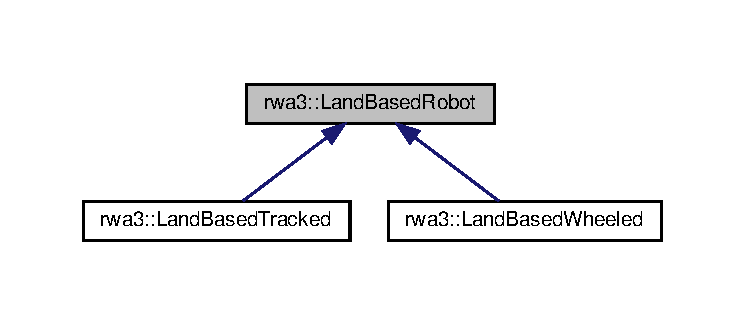
\includegraphics[width=350pt]{classrwa3_1_1_land_based_robot__inherit__graph}
\end{center}
\end{figure}
\subsection*{Public Member Functions}
\begin{DoxyCompactItemize}
\item 
\hyperlink{classrwa3_1_1_land_based_robot_abc40ff92063f51e3bf8ac8b7728ca12a}{Land\+Based\+Robot} (std\+::string name=\char`\"{}robot\char`\"{}, int x=0, int y=0)
\item 
virtual void \hyperlink{classrwa3_1_1_land_based_robot_a955b0741cce58648074edff80ac1ce29}{Go\+Up} (int x, int y)=0
\item 
virtual void \hyperlink{classrwa3_1_1_land_based_robot_a14fcb1b05297131cd09e8a57b8de0578}{Go\+Down} (int x, int y)=0
\item 
virtual void \hyperlink{classrwa3_1_1_land_based_robot_a9adfb103725320c1daff9ab72b0aad08}{Turn\+Left} (int x, int y)=0
\item 
virtual void \hyperlink{classrwa3_1_1_land_based_robot_ab62f4e787ae7f04dd9374b4f7e84985c}{Turn\+Right} (int x, int y)=0
\item 
virtual void \hyperlink{classrwa3_1_1_land_based_robot_adf0c76440e2f9d2ea5cbe7193cddfe2b}{Pick\+Up} (std\+::string obj)
\item 
virtual void \hyperlink{classrwa3_1_1_land_based_robot_a5cae9fc0c1365b984e09b807f79089e0}{Release} (std\+::string obj)
\item 
virtual int \hyperlink{classrwa3_1_1_land_based_robot_af47bec53268bd409305d2f97f45411ab}{get\+\_\+x} () const
\item 
virtual int \hyperlink{classrwa3_1_1_land_based_robot_a6de17dafe355573275264f74a59f974d}{get\+\_\+y} () const
\item 
virtual \hyperlink{classrwa3_1_1_land_based_robot_ac57e1fa6a06533403765c3ca0a7fc2d6}{$\sim$\+Land\+Based\+Robot} ()
\end{DoxyCompactItemize}
\subsection*{Protected Attributes}
\begin{DoxyCompactItemize}
\item 
const std\+::string \hyperlink{classrwa3_1_1_land_based_robot_aa633266ad18ca432217297f7caabbbe2}{name\+\_\+}
\item 
double \hyperlink{classrwa3_1_1_land_based_robot_ad9831c30393edcd779041734db24d819}{speed\+\_\+} \{\}
\item 
double \hyperlink{classrwa3_1_1_land_based_robot_a04a444830f3ad0c0d78d206e0d598bbb}{width\+\_\+} \{\}
\item 
double \hyperlink{classrwa3_1_1_land_based_robot_ac4b3cde4702d4ea866f503eedf6ea1e3}{length\+\_\+} \{\}
\item 
double \hyperlink{classrwa3_1_1_land_based_robot_a1187f7a4fd44450abf81a1ad76f18f72}{height\+\_\+} \{\}
\item 
double \hyperlink{classrwa3_1_1_land_based_robot_aa717b15025b339a0f40f689452a97cf8}{capacity\+\_\+} \{\}
\item 
int \hyperlink{classrwa3_1_1_land_based_robot_a832cf3ec3e8226a5dca17f2177a5730a}{x\+\_\+}
\item 
int \hyperlink{classrwa3_1_1_land_based_robot_a2749e5dd4c77633f72eba70d269fdf59}{y\+\_\+}
\end{DoxyCompactItemize}


\subsection{Detailed Description}


Definition at line 9 of file Land\+Based\+Robot.\+h.



\subsection{Constructor \& Destructor Documentation}
\mbox{\Hypertarget{classrwa3_1_1_land_based_robot_abc40ff92063f51e3bf8ac8b7728ca12a}\label{classrwa3_1_1_land_based_robot_abc40ff92063f51e3bf8ac8b7728ca12a}} 
\index{rwa3\+::\+Land\+Based\+Robot@{rwa3\+::\+Land\+Based\+Robot}!Land\+Based\+Robot@{Land\+Based\+Robot}}
\index{Land\+Based\+Robot@{Land\+Based\+Robot}!rwa3\+::\+Land\+Based\+Robot@{rwa3\+::\+Land\+Based\+Robot}}
\subsubsection{\texorpdfstring{Land\+Based\+Robot()}{LandBasedRobot()}}
{\footnotesize\ttfamily rwa3\+::\+Land\+Based\+Robot\+::\+Land\+Based\+Robot (\begin{DoxyParamCaption}\item[{std\+::string}]{name = {\ttfamily \char`\"{}robot\char`\"{}},  }\item[{int}]{x = {\ttfamily 0},  }\item[{int}]{y = {\ttfamily 0} }\end{DoxyParamCaption})\hspace{0.3cm}{\ttfamily [inline]}, {\ttfamily [explicit]}}

\hyperlink{classrwa3_1_1_land_based_robot}{Land\+Based\+Robot} Constructor 
\begin{DoxyParams}{Parameters}
{\em name} & name of the robot \\
\hline
{\em x} & x coordinate of the robot \\
\hline
{\em y} & y coordinate of the robot \\
\hline
\end{DoxyParams}


Definition at line 17 of file Land\+Based\+Robot.\+h.

\mbox{\Hypertarget{classrwa3_1_1_land_based_robot_ac57e1fa6a06533403765c3ca0a7fc2d6}\label{classrwa3_1_1_land_based_robot_ac57e1fa6a06533403765c3ca0a7fc2d6}} 
\index{rwa3\+::\+Land\+Based\+Robot@{rwa3\+::\+Land\+Based\+Robot}!````~Land\+Based\+Robot@{$\sim$\+Land\+Based\+Robot}}
\index{````~Land\+Based\+Robot@{$\sim$\+Land\+Based\+Robot}!rwa3\+::\+Land\+Based\+Robot@{rwa3\+::\+Land\+Based\+Robot}}
\subsubsection{\texorpdfstring{$\sim$\+Land\+Based\+Robot()}{~LandBasedRobot()}}
{\footnotesize\ttfamily virtual rwa3\+::\+Land\+Based\+Robot\+::$\sim$\+Land\+Based\+Robot (\begin{DoxyParamCaption}{ }\end{DoxyParamCaption})\hspace{0.3cm}{\ttfamily [inline]}, {\ttfamily [virtual]}}

Destructor for \hyperlink{classrwa3_1_1_land_based_robot}{Land\+Based\+Robot} 

Definition at line 77 of file Land\+Based\+Robot.\+h.



\subsection{Member Function Documentation}
\mbox{\Hypertarget{classrwa3_1_1_land_based_robot_af47bec53268bd409305d2f97f45411ab}\label{classrwa3_1_1_land_based_robot_af47bec53268bd409305d2f97f45411ab}} 
\index{rwa3\+::\+Land\+Based\+Robot@{rwa3\+::\+Land\+Based\+Robot}!get\+\_\+x@{get\+\_\+x}}
\index{get\+\_\+x@{get\+\_\+x}!rwa3\+::\+Land\+Based\+Robot@{rwa3\+::\+Land\+Based\+Robot}}
\subsubsection{\texorpdfstring{get\+\_\+x()}{get\_x()}}
{\footnotesize\ttfamily virtual int rwa3\+::\+Land\+Based\+Robot\+::get\+\_\+x (\begin{DoxyParamCaption}{ }\end{DoxyParamCaption}) const\hspace{0.3cm}{\ttfamily [inline]}, {\ttfamily [virtual]}}

Get the x coordinate of the robot \begin{DoxyReturn}{Returns}

\end{DoxyReturn}


Reimplemented in \hyperlink{classrwa3_1_1_land_based_tracked_a9065f381181bef7d8a4c8f4061ef2cda}{rwa3\+::\+Land\+Based\+Tracked}, and \hyperlink{classrwa3_1_1_land_based_wheeled_a71d85c53a65516d08728284e27107f65}{rwa3\+::\+Land\+Based\+Wheeled}.



Definition at line 65 of file Land\+Based\+Robot.\+h.

\mbox{\Hypertarget{classrwa3_1_1_land_based_robot_a6de17dafe355573275264f74a59f974d}\label{classrwa3_1_1_land_based_robot_a6de17dafe355573275264f74a59f974d}} 
\index{rwa3\+::\+Land\+Based\+Robot@{rwa3\+::\+Land\+Based\+Robot}!get\+\_\+y@{get\+\_\+y}}
\index{get\+\_\+y@{get\+\_\+y}!rwa3\+::\+Land\+Based\+Robot@{rwa3\+::\+Land\+Based\+Robot}}
\subsubsection{\texorpdfstring{get\+\_\+y()}{get\_y()}}
{\footnotesize\ttfamily virtual int rwa3\+::\+Land\+Based\+Robot\+::get\+\_\+y (\begin{DoxyParamCaption}{ }\end{DoxyParamCaption}) const\hspace{0.3cm}{\ttfamily [inline]}, {\ttfamily [virtual]}}

Get the y coordinate of the robot \begin{DoxyReturn}{Returns}

\end{DoxyReturn}


Reimplemented in \hyperlink{classrwa3_1_1_land_based_tracked_a11025bced4da296a2207e169fe328857}{rwa3\+::\+Land\+Based\+Tracked}, and \hyperlink{classrwa3_1_1_land_based_wheeled_ac16ccd003eae45997e00b4eee71bae3f}{rwa3\+::\+Land\+Based\+Wheeled}.



Definition at line 72 of file Land\+Based\+Robot.\+h.

\mbox{\Hypertarget{classrwa3_1_1_land_based_robot_a14fcb1b05297131cd09e8a57b8de0578}\label{classrwa3_1_1_land_based_robot_a14fcb1b05297131cd09e8a57b8de0578}} 
\index{rwa3\+::\+Land\+Based\+Robot@{rwa3\+::\+Land\+Based\+Robot}!Go\+Down@{Go\+Down}}
\index{Go\+Down@{Go\+Down}!rwa3\+::\+Land\+Based\+Robot@{rwa3\+::\+Land\+Based\+Robot}}
\subsubsection{\texorpdfstring{Go\+Down()}{GoDown()}}
{\footnotesize\ttfamily void rwa3\+::\+Land\+Based\+Robot\+::\+Go\+Down (\begin{DoxyParamCaption}\item[{int}]{x,  }\item[{int}]{y }\end{DoxyParamCaption})\hspace{0.3cm}{\ttfamily [pure virtual]}}

Virtual Go\+Down Method Moves the robot down in the maze 
\begin{DoxyParams}{Parameters}
{\em x} & x coordinate of the robot \\
\hline
{\em y} & y coordinate of the robot \\
\hline
\end{DoxyParams}


Implemented in \hyperlink{classrwa3_1_1_land_based_tracked_a1258bb7873abc517913e84e33effd6c4}{rwa3\+::\+Land\+Based\+Tracked}, and \hyperlink{classrwa3_1_1_land_based_wheeled_a20208be52afe9cdb302f288be3bb7608}{rwa3\+::\+Land\+Based\+Wheeled}.



Definition at line 9 of file Land\+Based\+Robot.\+cpp.

\mbox{\Hypertarget{classrwa3_1_1_land_based_robot_a955b0741cce58648074edff80ac1ce29}\label{classrwa3_1_1_land_based_robot_a955b0741cce58648074edff80ac1ce29}} 
\index{rwa3\+::\+Land\+Based\+Robot@{rwa3\+::\+Land\+Based\+Robot}!Go\+Up@{Go\+Up}}
\index{Go\+Up@{Go\+Up}!rwa3\+::\+Land\+Based\+Robot@{rwa3\+::\+Land\+Based\+Robot}}
\subsubsection{\texorpdfstring{Go\+Up()}{GoUp()}}
{\footnotesize\ttfamily void rwa3\+::\+Land\+Based\+Robot\+::\+Go\+Up (\begin{DoxyParamCaption}\item[{int}]{x,  }\item[{int}]{y }\end{DoxyParamCaption})\hspace{0.3cm}{\ttfamily [pure virtual]}}

Virtual Go\+Up Method Moves the robot up in the maze 
\begin{DoxyParams}{Parameters}
{\em x} & x coordinate of the robot \\
\hline
{\em y} & y coordinate of the robot \\
\hline
\end{DoxyParams}


Implemented in \hyperlink{classrwa3_1_1_land_based_tracked_a36d32a38c1c7cf44c5d7aebeb18f79ff}{rwa3\+::\+Land\+Based\+Tracked}, and \hyperlink{classrwa3_1_1_land_based_wheeled_a5feba1496039c50dd2d2f87fc286f438}{rwa3\+::\+Land\+Based\+Wheeled}.



Definition at line 5 of file Land\+Based\+Robot.\+cpp.

\mbox{\Hypertarget{classrwa3_1_1_land_based_robot_adf0c76440e2f9d2ea5cbe7193cddfe2b}\label{classrwa3_1_1_land_based_robot_adf0c76440e2f9d2ea5cbe7193cddfe2b}} 
\index{rwa3\+::\+Land\+Based\+Robot@{rwa3\+::\+Land\+Based\+Robot}!Pick\+Up@{Pick\+Up}}
\index{Pick\+Up@{Pick\+Up}!rwa3\+::\+Land\+Based\+Robot@{rwa3\+::\+Land\+Based\+Robot}}
\subsubsection{\texorpdfstring{Pick\+Up()}{PickUp()}}
{\footnotesize\ttfamily void rwa3\+::\+Land\+Based\+Robot\+::\+Pick\+Up (\begin{DoxyParamCaption}\item[{std\+::string}]{obj }\end{DoxyParamCaption})\hspace{0.3cm}{\ttfamily [virtual]}}

Virtual Pick\+Up Method Arm picks up an object 
\begin{DoxyParams}{Parameters}
{\em obj} & \\
\hline
\end{DoxyParams}


Reimplemented in \hyperlink{classrwa3_1_1_land_based_tracked_af1e65be827430cd9281e982409ebedcb}{rwa3\+::\+Land\+Based\+Tracked}, and \hyperlink{classrwa3_1_1_land_based_wheeled_aa82a9a72c4452ba203edc4c9ef0ad6c6}{rwa3\+::\+Land\+Based\+Wheeled}.



Definition at line 21 of file Land\+Based\+Robot.\+cpp.

\mbox{\Hypertarget{classrwa3_1_1_land_based_robot_a5cae9fc0c1365b984e09b807f79089e0}\label{classrwa3_1_1_land_based_robot_a5cae9fc0c1365b984e09b807f79089e0}} 
\index{rwa3\+::\+Land\+Based\+Robot@{rwa3\+::\+Land\+Based\+Robot}!Release@{Release}}
\index{Release@{Release}!rwa3\+::\+Land\+Based\+Robot@{rwa3\+::\+Land\+Based\+Robot}}
\subsubsection{\texorpdfstring{Release()}{Release()}}
{\footnotesize\ttfamily void rwa3\+::\+Land\+Based\+Robot\+::\+Release (\begin{DoxyParamCaption}\item[{std\+::string}]{obj }\end{DoxyParamCaption})\hspace{0.3cm}{\ttfamily [virtual]}}

Virtual Release Method Arm release an object 
\begin{DoxyParams}{Parameters}
{\em obj} & \\
\hline
\end{DoxyParams}


Reimplemented in \hyperlink{classrwa3_1_1_land_based_tracked_a89dbcac8ec2fd64c6b168167cd6363a4}{rwa3\+::\+Land\+Based\+Tracked}, and \hyperlink{classrwa3_1_1_land_based_wheeled_af4bd6e50a4a6d30186c969add4d9c954}{rwa3\+::\+Land\+Based\+Wheeled}.



Definition at line 25 of file Land\+Based\+Robot.\+cpp.

\mbox{\Hypertarget{classrwa3_1_1_land_based_robot_a9adfb103725320c1daff9ab72b0aad08}\label{classrwa3_1_1_land_based_robot_a9adfb103725320c1daff9ab72b0aad08}} 
\index{rwa3\+::\+Land\+Based\+Robot@{rwa3\+::\+Land\+Based\+Robot}!Turn\+Left@{Turn\+Left}}
\index{Turn\+Left@{Turn\+Left}!rwa3\+::\+Land\+Based\+Robot@{rwa3\+::\+Land\+Based\+Robot}}
\subsubsection{\texorpdfstring{Turn\+Left()}{TurnLeft()}}
{\footnotesize\ttfamily void rwa3\+::\+Land\+Based\+Robot\+::\+Turn\+Left (\begin{DoxyParamCaption}\item[{int}]{x,  }\item[{int}]{y }\end{DoxyParamCaption})\hspace{0.3cm}{\ttfamily [pure virtual]}}

Virtual Turn\+Left Method Moves the robot left in the maze 
\begin{DoxyParams}{Parameters}
{\em x} & x coordinate of the robot \\
\hline
{\em y} & y coordinate of the robot \\
\hline
\end{DoxyParams}


Implemented in \hyperlink{classrwa3_1_1_land_based_tracked_a6f8d74079ad047edd9f17cc541eafa86}{rwa3\+::\+Land\+Based\+Tracked}, and \hyperlink{classrwa3_1_1_land_based_wheeled_a5a659cca86a65e89156ef30ff363de41}{rwa3\+::\+Land\+Based\+Wheeled}.



Definition at line 13 of file Land\+Based\+Robot.\+cpp.

\mbox{\Hypertarget{classrwa3_1_1_land_based_robot_ab62f4e787ae7f04dd9374b4f7e84985c}\label{classrwa3_1_1_land_based_robot_ab62f4e787ae7f04dd9374b4f7e84985c}} 
\index{rwa3\+::\+Land\+Based\+Robot@{rwa3\+::\+Land\+Based\+Robot}!Turn\+Right@{Turn\+Right}}
\index{Turn\+Right@{Turn\+Right}!rwa3\+::\+Land\+Based\+Robot@{rwa3\+::\+Land\+Based\+Robot}}
\subsubsection{\texorpdfstring{Turn\+Right()}{TurnRight()}}
{\footnotesize\ttfamily void rwa3\+::\+Land\+Based\+Robot\+::\+Turn\+Right (\begin{DoxyParamCaption}\item[{int}]{x,  }\item[{int}]{y }\end{DoxyParamCaption})\hspace{0.3cm}{\ttfamily [pure virtual]}}

Virtual Turn\+Right Method Moves the robot right in the maze 
\begin{DoxyParams}{Parameters}
{\em x} & x coordinate of the robot \\
\hline
{\em y} & y coordinate of the robot \\
\hline
\end{DoxyParams}


Implemented in \hyperlink{classrwa3_1_1_land_based_tracked_a5f6a5b1871d9f75d8a724b8d7ae44d1f}{rwa3\+::\+Land\+Based\+Tracked}, and \hyperlink{classrwa3_1_1_land_based_wheeled_a90d9a8735197a7647f508c1983191590}{rwa3\+::\+Land\+Based\+Wheeled}.



Definition at line 17 of file Land\+Based\+Robot.\+cpp.



\subsection{Member Data Documentation}
\mbox{\Hypertarget{classrwa3_1_1_land_based_robot_aa717b15025b339a0f40f689452a97cf8}\label{classrwa3_1_1_land_based_robot_aa717b15025b339a0f40f689452a97cf8}} 
\index{rwa3\+::\+Land\+Based\+Robot@{rwa3\+::\+Land\+Based\+Robot}!capacity\+\_\+@{capacity\+\_\+}}
\index{capacity\+\_\+@{capacity\+\_\+}!rwa3\+::\+Land\+Based\+Robot@{rwa3\+::\+Land\+Based\+Robot}}
\subsubsection{\texorpdfstring{capacity\+\_\+}{capacity\_}}
{\footnotesize\ttfamily double rwa3\+::\+Land\+Based\+Robot\+::capacity\+\_\+ \{\}\hspace{0.3cm}{\ttfamily [protected]}}

Height of the base of the robot 

Definition at line 87 of file Land\+Based\+Robot.\+h.

\mbox{\Hypertarget{classrwa3_1_1_land_based_robot_a1187f7a4fd44450abf81a1ad76f18f72}\label{classrwa3_1_1_land_based_robot_a1187f7a4fd44450abf81a1ad76f18f72}} 
\index{rwa3\+::\+Land\+Based\+Robot@{rwa3\+::\+Land\+Based\+Robot}!height\+\_\+@{height\+\_\+}}
\index{height\+\_\+@{height\+\_\+}!rwa3\+::\+Land\+Based\+Robot@{rwa3\+::\+Land\+Based\+Robot}}
\subsubsection{\texorpdfstring{height\+\_\+}{height\_}}
{\footnotesize\ttfamily double rwa3\+::\+Land\+Based\+Robot\+::height\+\_\+ \{\}\hspace{0.3cm}{\ttfamily [protected]}}

Height of the base of the robot 

Definition at line 86 of file Land\+Based\+Robot.\+h.

\mbox{\Hypertarget{classrwa3_1_1_land_based_robot_ac4b3cde4702d4ea866f503eedf6ea1e3}\label{classrwa3_1_1_land_based_robot_ac4b3cde4702d4ea866f503eedf6ea1e3}} 
\index{rwa3\+::\+Land\+Based\+Robot@{rwa3\+::\+Land\+Based\+Robot}!length\+\_\+@{length\+\_\+}}
\index{length\+\_\+@{length\+\_\+}!rwa3\+::\+Land\+Based\+Robot@{rwa3\+::\+Land\+Based\+Robot}}
\subsubsection{\texorpdfstring{length\+\_\+}{length\_}}
{\footnotesize\ttfamily double rwa3\+::\+Land\+Based\+Robot\+::length\+\_\+ \{\}\hspace{0.3cm}{\ttfamily [protected]}}

Width of the base of the robot 

Definition at line 85 of file Land\+Based\+Robot.\+h.

\mbox{\Hypertarget{classrwa3_1_1_land_based_robot_aa633266ad18ca432217297f7caabbbe2}\label{classrwa3_1_1_land_based_robot_aa633266ad18ca432217297f7caabbbe2}} 
\index{rwa3\+::\+Land\+Based\+Robot@{rwa3\+::\+Land\+Based\+Robot}!name\+\_\+@{name\+\_\+}}
\index{name\+\_\+@{name\+\_\+}!rwa3\+::\+Land\+Based\+Robot@{rwa3\+::\+Land\+Based\+Robot}}
\subsubsection{\texorpdfstring{name\+\_\+}{name\_}}
{\footnotesize\ttfamily const std\+::string rwa3\+::\+Land\+Based\+Robot\+::name\+\_\+\hspace{0.3cm}{\ttfamily [protected]}}

Name of the robot 

Definition at line 79 of file Land\+Based\+Robot.\+h.

\mbox{\Hypertarget{classrwa3_1_1_land_based_robot_ad9831c30393edcd779041734db24d819}\label{classrwa3_1_1_land_based_robot_ad9831c30393edcd779041734db24d819}} 
\index{rwa3\+::\+Land\+Based\+Robot@{rwa3\+::\+Land\+Based\+Robot}!speed\+\_\+@{speed\+\_\+}}
\index{speed\+\_\+@{speed\+\_\+}!rwa3\+::\+Land\+Based\+Robot@{rwa3\+::\+Land\+Based\+Robot}}
\subsubsection{\texorpdfstring{speed\+\_\+}{speed\_}}
{\footnotesize\ttfamily double rwa3\+::\+Land\+Based\+Robot\+::speed\+\_\+ \{\}\hspace{0.3cm}{\ttfamily [protected]}}

Driving speed of the robot 

Definition at line 83 of file Land\+Based\+Robot.\+h.

\mbox{\Hypertarget{classrwa3_1_1_land_based_robot_a04a444830f3ad0c0d78d206e0d598bbb}\label{classrwa3_1_1_land_based_robot_a04a444830f3ad0c0d78d206e0d598bbb}} 
\index{rwa3\+::\+Land\+Based\+Robot@{rwa3\+::\+Land\+Based\+Robot}!width\+\_\+@{width\+\_\+}}
\index{width\+\_\+@{width\+\_\+}!rwa3\+::\+Land\+Based\+Robot@{rwa3\+::\+Land\+Based\+Robot}}
\subsubsection{\texorpdfstring{width\+\_\+}{width\_}}
{\footnotesize\ttfamily double rwa3\+::\+Land\+Based\+Robot\+::width\+\_\+ \{\}\hspace{0.3cm}{\ttfamily [protected]}}

Width of the base of the robot 

Definition at line 84 of file Land\+Based\+Robot.\+h.

\mbox{\Hypertarget{classrwa3_1_1_land_based_robot_a832cf3ec3e8226a5dca17f2177a5730a}\label{classrwa3_1_1_land_based_robot_a832cf3ec3e8226a5dca17f2177a5730a}} 
\index{rwa3\+::\+Land\+Based\+Robot@{rwa3\+::\+Land\+Based\+Robot}!x\+\_\+@{x\+\_\+}}
\index{x\+\_\+@{x\+\_\+}!rwa3\+::\+Land\+Based\+Robot@{rwa3\+::\+Land\+Based\+Robot}}
\subsubsection{\texorpdfstring{x\+\_\+}{x\_}}
{\footnotesize\ttfamily int rwa3\+::\+Land\+Based\+Robot\+::x\+\_\+\hspace{0.3cm}{\ttfamily [protected]}}

x coordinate of the robot 

Definition at line 88 of file Land\+Based\+Robot.\+h.

\mbox{\Hypertarget{classrwa3_1_1_land_based_robot_a2749e5dd4c77633f72eba70d269fdf59}\label{classrwa3_1_1_land_based_robot_a2749e5dd4c77633f72eba70d269fdf59}} 
\index{rwa3\+::\+Land\+Based\+Robot@{rwa3\+::\+Land\+Based\+Robot}!y\+\_\+@{y\+\_\+}}
\index{y\+\_\+@{y\+\_\+}!rwa3\+::\+Land\+Based\+Robot@{rwa3\+::\+Land\+Based\+Robot}}
\subsubsection{\texorpdfstring{y\+\_\+}{y\_}}
{\footnotesize\ttfamily int rwa3\+::\+Land\+Based\+Robot\+::y\+\_\+\hspace{0.3cm}{\ttfamily [protected]}}

y coordinate of the robot 

Definition at line 89 of file Land\+Based\+Robot.\+h.



The documentation for this class was generated from the following files\+:\begin{DoxyCompactItemize}
\item 
/home/diane/\+One\+Drive/\+Fall 2020/\+E\+N\+P\+M809\+Y Intro Robot Programming/\+Homework/\+R\+W\+A3-\/\+Group3/\+Land\+Based\+Robot/\hyperlink{_land_based_robot_8h}{Land\+Based\+Robot.\+h}\item 
/home/diane/\+One\+Drive/\+Fall 2020/\+E\+N\+P\+M809\+Y Intro Robot Programming/\+Homework/\+R\+W\+A3-\/\+Group3/\+Land\+Based\+Robot/\hyperlink{_land_based_robot_8cpp}{Land\+Based\+Robot.\+cpp}\end{DoxyCompactItemize}

\hypertarget{classrwa3_1_1_land_based_tracked}{}\section{rwa3\+:\+:Land\+Based\+Tracked Class Reference}
\label{classrwa3_1_1_land_based_tracked}\index{rwa3\+::\+Land\+Based\+Tracked@{rwa3\+::\+Land\+Based\+Tracked}}


{\ttfamily \#include $<$landbasedtracked.\+h$>$}



Inheritance diagram for rwa3\+:\+:Land\+Based\+Tracked\+:\nopagebreak
\begin{figure}[H]
\begin{center}
\leavevmode
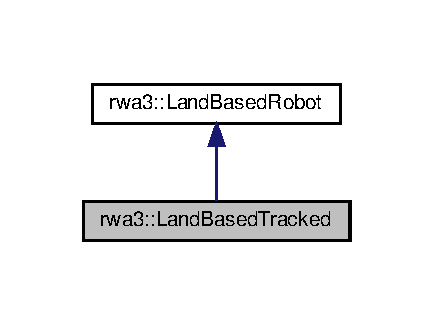
\includegraphics[width=208pt]{classrwa3_1_1_land_based_tracked__inherit__graph}
\end{center}
\end{figure}


Collaboration diagram for rwa3\+:\+:Land\+Based\+Tracked\+:\nopagebreak
\begin{figure}[H]
\begin{center}
\leavevmode
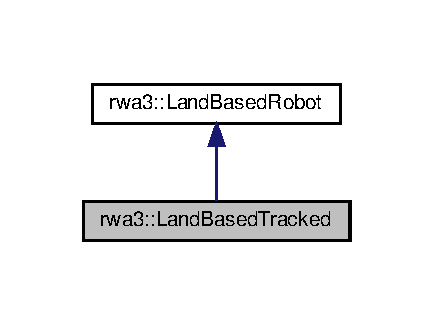
\includegraphics[width=208pt]{classrwa3_1_1_land_based_tracked__coll__graph}
\end{center}
\end{figure}
\subsection*{Public Member Functions}
\begin{DoxyCompactItemize}
\item 
\hyperlink{classrwa3_1_1_land_based_tracked_a7afa1f901374a08d0bb23882988eef46}{Land\+Based\+Tracked} (std\+::string name=\char`\"{}tracked\char`\"{}, int x=2, int y=3)
\item 
void \hyperlink{classrwa3_1_1_land_based_tracked_a36d32a38c1c7cf44c5d7aebeb18f79ff}{Go\+Up} (int x, int y) override
\item 
void \hyperlink{classrwa3_1_1_land_based_tracked_a1258bb7873abc517913e84e33effd6c4}{Go\+Down} (int x, int y) override
\item 
void \hyperlink{classrwa3_1_1_land_based_tracked_a6f8d74079ad047edd9f17cc541eafa86}{Turn\+Left} (int x, int y) override
\item 
void \hyperlink{classrwa3_1_1_land_based_tracked_a5f6a5b1871d9f75d8a724b8d7ae44d1f}{Turn\+Right} (int x, int y) override
\item 
void \hyperlink{classrwa3_1_1_land_based_tracked_af1e65be827430cd9281e982409ebedcb}{Pick\+Up} (std\+::string obj) override
\item 
void \hyperlink{classrwa3_1_1_land_based_tracked_a89dbcac8ec2fd64c6b168167cd6363a4}{Release} (std\+::string obj) override
\item 
int \hyperlink{classrwa3_1_1_land_based_tracked_a9065f381181bef7d8a4c8f4061ef2cda}{get\+\_\+x} () const
\item 
int \hyperlink{classrwa3_1_1_land_based_tracked_a11025bced4da296a2207e169fe328857}{get\+\_\+y} () const
\item 
virtual \hyperlink{classrwa3_1_1_land_based_tracked_a018639eac0eabfcf86fc2b48e0b6df83}{$\sim$\+Land\+Based\+Tracked} ()
\end{DoxyCompactItemize}
\subsection*{Protected Attributes}
\begin{DoxyCompactItemize}
\item 
std\+::shared\+\_\+ptr$<$ std\+::string $>$ \hyperlink{classrwa3_1_1_land_based_tracked_ae57d4a2861a045e2f0cc0da1e43868ed}{track\+\_\+type}
\item 
const std\+::string \hyperlink{classrwa3_1_1_land_based_tracked_ad7f474b8339e04a7b8a174b2366aee1b}{name\+\_\+}
\item 
double \hyperlink{classrwa3_1_1_land_based_tracked_a2bc2f3ff33c23a6eca670f2ee347508e}{speed\+\_\+} \{\}
\item 
double \hyperlink{classrwa3_1_1_land_based_tracked_a61f588ad9505ec4774568327620fba53}{width\+\_\+} \{\}
\item 
double \hyperlink{classrwa3_1_1_land_based_tracked_aa97c13720453621211935e0e96ba3790}{length\+\_\+} \{\}
\item 
double \hyperlink{classrwa3_1_1_land_based_tracked_a5e829ff7fae33fb1c29f5897c09311c8}{height\+\_\+} \{\}
\item 
double \hyperlink{classrwa3_1_1_land_based_tracked_a5b9e38961ec5d2850b9bd069e897f3cd}{capacity\+\_\+} \{\}
\item 
int \hyperlink{classrwa3_1_1_land_based_tracked_ad52ad096c20dd018142510ce1a872ba6}{x\+\_\+}
\item 
int \hyperlink{classrwa3_1_1_land_based_tracked_aa6273b2cfff5572934f132cf0ada463e}{y\+\_\+}
\end{DoxyCompactItemize}


\subsection{Detailed Description}


Definition at line 10 of file landbasedtracked.\+h.



\subsection{Constructor \& Destructor Documentation}
\mbox{\Hypertarget{classrwa3_1_1_land_based_tracked_a7afa1f901374a08d0bb23882988eef46}\label{classrwa3_1_1_land_based_tracked_a7afa1f901374a08d0bb23882988eef46}} 
\index{rwa3\+::\+Land\+Based\+Tracked@{rwa3\+::\+Land\+Based\+Tracked}!Land\+Based\+Tracked@{Land\+Based\+Tracked}}
\index{Land\+Based\+Tracked@{Land\+Based\+Tracked}!rwa3\+::\+Land\+Based\+Tracked@{rwa3\+::\+Land\+Based\+Tracked}}
\subsubsection{\texorpdfstring{Land\+Based\+Tracked()}{LandBasedTracked()}}
{\footnotesize\ttfamily rwa3\+::\+Land\+Based\+Tracked\+::\+Land\+Based\+Tracked (\begin{DoxyParamCaption}\item[{std\+::string}]{name = {\ttfamily \char`\"{}tracked\char`\"{}},  }\item[{int}]{x = {\ttfamily 2},  }\item[{int}]{y = {\ttfamily 3} }\end{DoxyParamCaption})\hspace{0.3cm}{\ttfamily [inline]}, {\ttfamily [explicit]}}

\hyperlink{classrwa3_1_1_land_based_tracked}{Land\+Based\+Tracked} Constructor 
\begin{DoxyParams}{Parameters}
{\em name} & name of the robot \\
\hline
{\em x} & x coordinate of the robot \\
\hline
{\em y} & y coordinate of the robot \\
\hline
\end{DoxyParams}


Definition at line 18 of file landbasedtracked.\+h.

\mbox{\Hypertarget{classrwa3_1_1_land_based_tracked_a018639eac0eabfcf86fc2b48e0b6df83}\label{classrwa3_1_1_land_based_tracked_a018639eac0eabfcf86fc2b48e0b6df83}} 
\index{rwa3\+::\+Land\+Based\+Tracked@{rwa3\+::\+Land\+Based\+Tracked}!````~Land\+Based\+Tracked@{$\sim$\+Land\+Based\+Tracked}}
\index{````~Land\+Based\+Tracked@{$\sim$\+Land\+Based\+Tracked}!rwa3\+::\+Land\+Based\+Tracked@{rwa3\+::\+Land\+Based\+Tracked}}
\subsubsection{\texorpdfstring{$\sim$\+Land\+Based\+Tracked()}{~LandBasedTracked()}}
{\footnotesize\ttfamily virtual rwa3\+::\+Land\+Based\+Tracked\+::$\sim$\+Land\+Based\+Tracked (\begin{DoxyParamCaption}{ }\end{DoxyParamCaption})\hspace{0.3cm}{\ttfamily [inline]}, {\ttfamily [virtual]}}

Destructor for \hyperlink{classrwa3_1_1_land_based_tracked}{Land\+Based\+Tracked} 

Definition at line 79 of file landbasedtracked.\+h.



\subsection{Member Function Documentation}
\mbox{\Hypertarget{classrwa3_1_1_land_based_tracked_a9065f381181bef7d8a4c8f4061ef2cda}\label{classrwa3_1_1_land_based_tracked_a9065f381181bef7d8a4c8f4061ef2cda}} 
\index{rwa3\+::\+Land\+Based\+Tracked@{rwa3\+::\+Land\+Based\+Tracked}!get\+\_\+x@{get\+\_\+x}}
\index{get\+\_\+x@{get\+\_\+x}!rwa3\+::\+Land\+Based\+Tracked@{rwa3\+::\+Land\+Based\+Tracked}}
\subsubsection{\texorpdfstring{get\+\_\+x()}{get\_x()}}
{\footnotesize\ttfamily int rwa3\+::\+Land\+Based\+Tracked\+::get\+\_\+x (\begin{DoxyParamCaption}{ }\end{DoxyParamCaption}) const\hspace{0.3cm}{\ttfamily [inline]}, {\ttfamily [virtual]}}

Get the x coordinate of the robot \begin{DoxyReturn}{Returns}

\end{DoxyReturn}


Reimplemented from \hyperlink{classrwa3_1_1_land_based_robot_af47bec53268bd409305d2f97f45411ab}{rwa3\+::\+Land\+Based\+Robot}.



Definition at line 68 of file landbasedtracked.\+h.

\mbox{\Hypertarget{classrwa3_1_1_land_based_tracked_a11025bced4da296a2207e169fe328857}\label{classrwa3_1_1_land_based_tracked_a11025bced4da296a2207e169fe328857}} 
\index{rwa3\+::\+Land\+Based\+Tracked@{rwa3\+::\+Land\+Based\+Tracked}!get\+\_\+y@{get\+\_\+y}}
\index{get\+\_\+y@{get\+\_\+y}!rwa3\+::\+Land\+Based\+Tracked@{rwa3\+::\+Land\+Based\+Tracked}}
\subsubsection{\texorpdfstring{get\+\_\+y()}{get\_y()}}
{\footnotesize\ttfamily int rwa3\+::\+Land\+Based\+Tracked\+::get\+\_\+y (\begin{DoxyParamCaption}{ }\end{DoxyParamCaption}) const\hspace{0.3cm}{\ttfamily [inline]}, {\ttfamily [virtual]}}

Get the y coordinate of the robot \begin{DoxyReturn}{Returns}

\end{DoxyReturn}


Reimplemented from \hyperlink{classrwa3_1_1_land_based_robot_a6de17dafe355573275264f74a59f974d}{rwa3\+::\+Land\+Based\+Robot}.



Definition at line 75 of file landbasedtracked.\+h.

\mbox{\Hypertarget{classrwa3_1_1_land_based_tracked_a1258bb7873abc517913e84e33effd6c4}\label{classrwa3_1_1_land_based_tracked_a1258bb7873abc517913e84e33effd6c4}} 
\index{rwa3\+::\+Land\+Based\+Tracked@{rwa3\+::\+Land\+Based\+Tracked}!Go\+Down@{Go\+Down}}
\index{Go\+Down@{Go\+Down}!rwa3\+::\+Land\+Based\+Tracked@{rwa3\+::\+Land\+Based\+Tracked}}
\subsubsection{\texorpdfstring{Go\+Down()}{GoDown()}}
{\footnotesize\ttfamily void rwa3\+::\+Land\+Based\+Tracked\+::\+Go\+Down (\begin{DoxyParamCaption}\item[{int}]{x,  }\item[{int}]{y }\end{DoxyParamCaption})\hspace{0.3cm}{\ttfamily [override]}, {\ttfamily [virtual]}}

Virtual Go\+Down Method Moves the robot down in the maze 
\begin{DoxyParams}{Parameters}
{\em x} & x coordinate of the robot \\
\hline
{\em y} & y coordinate of the robot \\
\hline
\end{DoxyParams}


Implements \hyperlink{classrwa3_1_1_land_based_robot_a14fcb1b05297131cd09e8a57b8de0578}{rwa3\+::\+Land\+Based\+Robot}.



Definition at line 11 of file landbasedtracked.\+cpp.

\mbox{\Hypertarget{classrwa3_1_1_land_based_tracked_a36d32a38c1c7cf44c5d7aebeb18f79ff}\label{classrwa3_1_1_land_based_tracked_a36d32a38c1c7cf44c5d7aebeb18f79ff}} 
\index{rwa3\+::\+Land\+Based\+Tracked@{rwa3\+::\+Land\+Based\+Tracked}!Go\+Up@{Go\+Up}}
\index{Go\+Up@{Go\+Up}!rwa3\+::\+Land\+Based\+Tracked@{rwa3\+::\+Land\+Based\+Tracked}}
\subsubsection{\texorpdfstring{Go\+Up()}{GoUp()}}
{\footnotesize\ttfamily void rwa3\+::\+Land\+Based\+Tracked\+::\+Go\+Up (\begin{DoxyParamCaption}\item[{int}]{x,  }\item[{int}]{y }\end{DoxyParamCaption})\hspace{0.3cm}{\ttfamily [override]}, {\ttfamily [virtual]}}

Virtual Go\+Up Method Moves the robot up in the maze 
\begin{DoxyParams}{Parameters}
{\em x} & x coordinate of the robot \\
\hline
{\em y} & y coordinate of the robot \\
\hline
\end{DoxyParams}


Implements \hyperlink{classrwa3_1_1_land_based_robot_a955b0741cce58648074edff80ac1ce29}{rwa3\+::\+Land\+Based\+Robot}.



Definition at line 7 of file landbasedtracked.\+cpp.

\mbox{\Hypertarget{classrwa3_1_1_land_based_tracked_af1e65be827430cd9281e982409ebedcb}\label{classrwa3_1_1_land_based_tracked_af1e65be827430cd9281e982409ebedcb}} 
\index{rwa3\+::\+Land\+Based\+Tracked@{rwa3\+::\+Land\+Based\+Tracked}!Pick\+Up@{Pick\+Up}}
\index{Pick\+Up@{Pick\+Up}!rwa3\+::\+Land\+Based\+Tracked@{rwa3\+::\+Land\+Based\+Tracked}}
\subsubsection{\texorpdfstring{Pick\+Up()}{PickUp()}}
{\footnotesize\ttfamily void rwa3\+::\+Land\+Based\+Tracked\+::\+Pick\+Up (\begin{DoxyParamCaption}\item[{std\+::string}]{obj }\end{DoxyParamCaption})\hspace{0.3cm}{\ttfamily [override]}, {\ttfamily [virtual]}}

Virtual Pick\+Up Method Arm picks up an object 
\begin{DoxyParams}{Parameters}
{\em obj} & \\
\hline
\end{DoxyParams}


Reimplemented from \hyperlink{classrwa3_1_1_land_based_robot_adf0c76440e2f9d2ea5cbe7193cddfe2b}{rwa3\+::\+Land\+Based\+Robot}.



Definition at line 23 of file landbasedtracked.\+cpp.

\mbox{\Hypertarget{classrwa3_1_1_land_based_tracked_a89dbcac8ec2fd64c6b168167cd6363a4}\label{classrwa3_1_1_land_based_tracked_a89dbcac8ec2fd64c6b168167cd6363a4}} 
\index{rwa3\+::\+Land\+Based\+Tracked@{rwa3\+::\+Land\+Based\+Tracked}!Release@{Release}}
\index{Release@{Release}!rwa3\+::\+Land\+Based\+Tracked@{rwa3\+::\+Land\+Based\+Tracked}}
\subsubsection{\texorpdfstring{Release()}{Release()}}
{\footnotesize\ttfamily void rwa3\+::\+Land\+Based\+Tracked\+::\+Release (\begin{DoxyParamCaption}\item[{std\+::string}]{obj }\end{DoxyParamCaption})\hspace{0.3cm}{\ttfamily [override]}, {\ttfamily [virtual]}}

Virtual Release Method Arm release an object 
\begin{DoxyParams}{Parameters}
{\em obj} & \\
\hline
\end{DoxyParams}


Reimplemented from \hyperlink{classrwa3_1_1_land_based_robot_a5cae9fc0c1365b984e09b807f79089e0}{rwa3\+::\+Land\+Based\+Robot}.



Definition at line 27 of file landbasedtracked.\+cpp.

\mbox{\Hypertarget{classrwa3_1_1_land_based_tracked_a6f8d74079ad047edd9f17cc541eafa86}\label{classrwa3_1_1_land_based_tracked_a6f8d74079ad047edd9f17cc541eafa86}} 
\index{rwa3\+::\+Land\+Based\+Tracked@{rwa3\+::\+Land\+Based\+Tracked}!Turn\+Left@{Turn\+Left}}
\index{Turn\+Left@{Turn\+Left}!rwa3\+::\+Land\+Based\+Tracked@{rwa3\+::\+Land\+Based\+Tracked}}
\subsubsection{\texorpdfstring{Turn\+Left()}{TurnLeft()}}
{\footnotesize\ttfamily void rwa3\+::\+Land\+Based\+Tracked\+::\+Turn\+Left (\begin{DoxyParamCaption}\item[{int}]{x,  }\item[{int}]{y }\end{DoxyParamCaption})\hspace{0.3cm}{\ttfamily [override]}, {\ttfamily [virtual]}}

Virtual Turn\+Left Method Moves the robot left in the maze 
\begin{DoxyParams}{Parameters}
{\em x} & x coordinate of the robot \\
\hline
{\em y} & y coordinate of the robot \\
\hline
\end{DoxyParams}


Implements \hyperlink{classrwa3_1_1_land_based_robot_a9adfb103725320c1daff9ab72b0aad08}{rwa3\+::\+Land\+Based\+Robot}.



Definition at line 15 of file landbasedtracked.\+cpp.

\mbox{\Hypertarget{classrwa3_1_1_land_based_tracked_a5f6a5b1871d9f75d8a724b8d7ae44d1f}\label{classrwa3_1_1_land_based_tracked_a5f6a5b1871d9f75d8a724b8d7ae44d1f}} 
\index{rwa3\+::\+Land\+Based\+Tracked@{rwa3\+::\+Land\+Based\+Tracked}!Turn\+Right@{Turn\+Right}}
\index{Turn\+Right@{Turn\+Right}!rwa3\+::\+Land\+Based\+Tracked@{rwa3\+::\+Land\+Based\+Tracked}}
\subsubsection{\texorpdfstring{Turn\+Right()}{TurnRight()}}
{\footnotesize\ttfamily void rwa3\+::\+Land\+Based\+Tracked\+::\+Turn\+Right (\begin{DoxyParamCaption}\item[{int}]{x,  }\item[{int}]{y }\end{DoxyParamCaption})\hspace{0.3cm}{\ttfamily [override]}, {\ttfamily [virtual]}}

Virtual Turn\+Right Method Moves the robot right in the maze 
\begin{DoxyParams}{Parameters}
{\em x} & x coordinate of the robot \\
\hline
{\em y} & y coordinate of the robot \\
\hline
\end{DoxyParams}


Implements \hyperlink{classrwa3_1_1_land_based_robot_ab62f4e787ae7f04dd9374b4f7e84985c}{rwa3\+::\+Land\+Based\+Robot}.



Definition at line 19 of file landbasedtracked.\+cpp.



\subsection{Member Data Documentation}
\mbox{\Hypertarget{classrwa3_1_1_land_based_tracked_a5b9e38961ec5d2850b9bd069e897f3cd}\label{classrwa3_1_1_land_based_tracked_a5b9e38961ec5d2850b9bd069e897f3cd}} 
\index{rwa3\+::\+Land\+Based\+Tracked@{rwa3\+::\+Land\+Based\+Tracked}!capacity\+\_\+@{capacity\+\_\+}}
\index{capacity\+\_\+@{capacity\+\_\+}!rwa3\+::\+Land\+Based\+Tracked@{rwa3\+::\+Land\+Based\+Tracked}}
\subsubsection{\texorpdfstring{capacity\+\_\+}{capacity\_}}
{\footnotesize\ttfamily double rwa3\+::\+Land\+Based\+Tracked\+::capacity\+\_\+ \{\}\hspace{0.3cm}{\ttfamily [protected]}}

Height of the base of the robot 

Definition at line 90 of file landbasedtracked.\+h.

\mbox{\Hypertarget{classrwa3_1_1_land_based_tracked_a5e829ff7fae33fb1c29f5897c09311c8}\label{classrwa3_1_1_land_based_tracked_a5e829ff7fae33fb1c29f5897c09311c8}} 
\index{rwa3\+::\+Land\+Based\+Tracked@{rwa3\+::\+Land\+Based\+Tracked}!height\+\_\+@{height\+\_\+}}
\index{height\+\_\+@{height\+\_\+}!rwa3\+::\+Land\+Based\+Tracked@{rwa3\+::\+Land\+Based\+Tracked}}
\subsubsection{\texorpdfstring{height\+\_\+}{height\_}}
{\footnotesize\ttfamily double rwa3\+::\+Land\+Based\+Tracked\+::height\+\_\+ \{\}\hspace{0.3cm}{\ttfamily [protected]}}

Height of the base of the robot 

Definition at line 89 of file landbasedtracked.\+h.

\mbox{\Hypertarget{classrwa3_1_1_land_based_tracked_aa97c13720453621211935e0e96ba3790}\label{classrwa3_1_1_land_based_tracked_aa97c13720453621211935e0e96ba3790}} 
\index{rwa3\+::\+Land\+Based\+Tracked@{rwa3\+::\+Land\+Based\+Tracked}!length\+\_\+@{length\+\_\+}}
\index{length\+\_\+@{length\+\_\+}!rwa3\+::\+Land\+Based\+Tracked@{rwa3\+::\+Land\+Based\+Tracked}}
\subsubsection{\texorpdfstring{length\+\_\+}{length\_}}
{\footnotesize\ttfamily double rwa3\+::\+Land\+Based\+Tracked\+::length\+\_\+ \{\}\hspace{0.3cm}{\ttfamily [protected]}}

Width of the base of the robot 

Definition at line 88 of file landbasedtracked.\+h.

\mbox{\Hypertarget{classrwa3_1_1_land_based_tracked_ad7f474b8339e04a7b8a174b2366aee1b}\label{classrwa3_1_1_land_based_tracked_ad7f474b8339e04a7b8a174b2366aee1b}} 
\index{rwa3\+::\+Land\+Based\+Tracked@{rwa3\+::\+Land\+Based\+Tracked}!name\+\_\+@{name\+\_\+}}
\index{name\+\_\+@{name\+\_\+}!rwa3\+::\+Land\+Based\+Tracked@{rwa3\+::\+Land\+Based\+Tracked}}
\subsubsection{\texorpdfstring{name\+\_\+}{name\_}}
{\footnotesize\ttfamily const std\+::string rwa3\+::\+Land\+Based\+Tracked\+::name\+\_\+\hspace{0.3cm}{\ttfamily [protected]}}

Type of track mounted on the robot Name of the robot 

Definition at line 85 of file landbasedtracked.\+h.

\mbox{\Hypertarget{classrwa3_1_1_land_based_tracked_a2bc2f3ff33c23a6eca670f2ee347508e}\label{classrwa3_1_1_land_based_tracked_a2bc2f3ff33c23a6eca670f2ee347508e}} 
\index{rwa3\+::\+Land\+Based\+Tracked@{rwa3\+::\+Land\+Based\+Tracked}!speed\+\_\+@{speed\+\_\+}}
\index{speed\+\_\+@{speed\+\_\+}!rwa3\+::\+Land\+Based\+Tracked@{rwa3\+::\+Land\+Based\+Tracked}}
\subsubsection{\texorpdfstring{speed\+\_\+}{speed\_}}
{\footnotesize\ttfamily double rwa3\+::\+Land\+Based\+Tracked\+::speed\+\_\+ \{\}\hspace{0.3cm}{\ttfamily [protected]}}

Driving speed of the robot 

Definition at line 86 of file landbasedtracked.\+h.

\mbox{\Hypertarget{classrwa3_1_1_land_based_tracked_ae57d4a2861a045e2f0cc0da1e43868ed}\label{classrwa3_1_1_land_based_tracked_ae57d4a2861a045e2f0cc0da1e43868ed}} 
\index{rwa3\+::\+Land\+Based\+Tracked@{rwa3\+::\+Land\+Based\+Tracked}!track\+\_\+type@{track\+\_\+type}}
\index{track\+\_\+type@{track\+\_\+type}!rwa3\+::\+Land\+Based\+Tracked@{rwa3\+::\+Land\+Based\+Tracked}}
\subsubsection{\texorpdfstring{track\+\_\+type}{track\_type}}
{\footnotesize\ttfamily std\+::shared\+\_\+ptr$<$std\+::string$>$ rwa3\+::\+Land\+Based\+Tracked\+::track\+\_\+type\hspace{0.3cm}{\ttfamily [protected]}}



Definition at line 81 of file landbasedtracked.\+h.

\mbox{\Hypertarget{classrwa3_1_1_land_based_tracked_a61f588ad9505ec4774568327620fba53}\label{classrwa3_1_1_land_based_tracked_a61f588ad9505ec4774568327620fba53}} 
\index{rwa3\+::\+Land\+Based\+Tracked@{rwa3\+::\+Land\+Based\+Tracked}!width\+\_\+@{width\+\_\+}}
\index{width\+\_\+@{width\+\_\+}!rwa3\+::\+Land\+Based\+Tracked@{rwa3\+::\+Land\+Based\+Tracked}}
\subsubsection{\texorpdfstring{width\+\_\+}{width\_}}
{\footnotesize\ttfamily double rwa3\+::\+Land\+Based\+Tracked\+::width\+\_\+ \{\}\hspace{0.3cm}{\ttfamily [protected]}}

Width of the base of the robot 

Definition at line 87 of file landbasedtracked.\+h.

\mbox{\Hypertarget{classrwa3_1_1_land_based_tracked_ad52ad096c20dd018142510ce1a872ba6}\label{classrwa3_1_1_land_based_tracked_ad52ad096c20dd018142510ce1a872ba6}} 
\index{rwa3\+::\+Land\+Based\+Tracked@{rwa3\+::\+Land\+Based\+Tracked}!x\+\_\+@{x\+\_\+}}
\index{x\+\_\+@{x\+\_\+}!rwa3\+::\+Land\+Based\+Tracked@{rwa3\+::\+Land\+Based\+Tracked}}
\subsubsection{\texorpdfstring{x\+\_\+}{x\_}}
{\footnotesize\ttfamily int rwa3\+::\+Land\+Based\+Tracked\+::x\+\_\+\hspace{0.3cm}{\ttfamily [protected]}}

x coordinate of the robot 

Definition at line 91 of file landbasedtracked.\+h.

\mbox{\Hypertarget{classrwa3_1_1_land_based_tracked_aa6273b2cfff5572934f132cf0ada463e}\label{classrwa3_1_1_land_based_tracked_aa6273b2cfff5572934f132cf0ada463e}} 
\index{rwa3\+::\+Land\+Based\+Tracked@{rwa3\+::\+Land\+Based\+Tracked}!y\+\_\+@{y\+\_\+}}
\index{y\+\_\+@{y\+\_\+}!rwa3\+::\+Land\+Based\+Tracked@{rwa3\+::\+Land\+Based\+Tracked}}
\subsubsection{\texorpdfstring{y\+\_\+}{y\_}}
{\footnotesize\ttfamily int rwa3\+::\+Land\+Based\+Tracked\+::y\+\_\+\hspace{0.3cm}{\ttfamily [protected]}}

y coordinate of the robot 

Definition at line 92 of file landbasedtracked.\+h.



The documentation for this class was generated from the following files\+:\begin{DoxyCompactItemize}
\item 
/home/diane/\+One\+Drive/\+Fall 2020/\+E\+N\+P\+M809\+Y Intro Robot Programming/\+Homework/\+R\+W\+A3-\/\+Group3/\+Land\+Based\+Tracked/\hyperlink{landbasedtracked_8h}{landbasedtracked.\+h}\item 
/home/diane/\+One\+Drive/\+Fall 2020/\+E\+N\+P\+M809\+Y Intro Robot Programming/\+Homework/\+R\+W\+A3-\/\+Group3/\+Land\+Based\+Tracked/\hyperlink{landbasedtracked_8cpp}{landbasedtracked.\+cpp}\end{DoxyCompactItemize}

\hypertarget{classrwa3_1_1_land_based_wheeled}{}\section{rwa3\+:\+:Land\+Based\+Wheeled Class Reference}
\label{classrwa3_1_1_land_based_wheeled}\index{rwa3\+::\+Land\+Based\+Wheeled@{rwa3\+::\+Land\+Based\+Wheeled}}


{\ttfamily \#include $<$landbasedwheeled.\+h$>$}



Inheritance diagram for rwa3\+:\+:Land\+Based\+Wheeled\+:\nopagebreak
\begin{figure}[H]
\begin{center}
\leavevmode
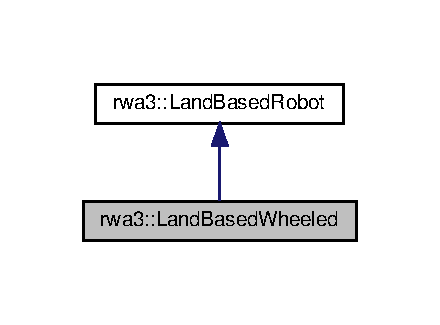
\includegraphics[width=211pt]{classrwa3_1_1_land_based_wheeled__inherit__graph}
\end{center}
\end{figure}


Collaboration diagram for rwa3\+:\+:Land\+Based\+Wheeled\+:\nopagebreak
\begin{figure}[H]
\begin{center}
\leavevmode
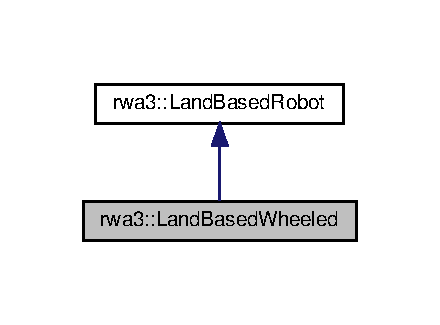
\includegraphics[width=211pt]{classrwa3_1_1_land_based_wheeled__coll__graph}
\end{center}
\end{figure}
\subsection*{Public Member Functions}
\begin{DoxyCompactItemize}
\item 
\hyperlink{classrwa3_1_1_land_based_wheeled_a0a8f57819c36e24c6b2320d8088919af}{Land\+Based\+Wheeled} (std\+::string name=\char`\"{}wheeled\char`\"{}, int x=1, int y=4, int wheels=4)
\item 
void \hyperlink{classrwa3_1_1_land_based_wheeled_a5feba1496039c50dd2d2f87fc286f438}{Go\+Up} (int x, int y) override
\item 
void \hyperlink{classrwa3_1_1_land_based_wheeled_a20208be52afe9cdb302f288be3bb7608}{Go\+Down} (int x, int y) override
\item 
void \hyperlink{classrwa3_1_1_land_based_wheeled_a5a659cca86a65e89156ef30ff363de41}{Turn\+Left} (int x, int y) override
\item 
void \hyperlink{classrwa3_1_1_land_based_wheeled_a90d9a8735197a7647f508c1983191590}{Turn\+Right} (int x, int y) override
\item 
void \hyperlink{classrwa3_1_1_land_based_wheeled_aa82a9a72c4452ba203edc4c9ef0ad6c6}{Pick\+Up} (std\+::string obj) override
\item 
void \hyperlink{classrwa3_1_1_land_based_wheeled_af4bd6e50a4a6d30186c969add4d9c954}{Release} (std\+::string obj) override
\item 
int \hyperlink{classrwa3_1_1_land_based_wheeled_a71d85c53a65516d08728284e27107f65}{get\+\_\+x} () const
\item 
int \hyperlink{classrwa3_1_1_land_based_wheeled_ac16ccd003eae45997e00b4eee71bae3f}{get\+\_\+y} () const
\item 
virtual \hyperlink{classrwa3_1_1_land_based_wheeled_a0c46a810956dbe99d0a94db8d238d4d7}{$\sim$\+Land\+Based\+Wheeled} ()
\end{DoxyCompactItemize}
\subsection*{Protected Attributes}
\begin{DoxyCompactItemize}
\item 
const int \hyperlink{classrwa3_1_1_land_based_wheeled_a99064bf2a79b4c18eb43810434ed934d}{wheel\+\_\+number}
\item 
std\+::shared\+\_\+ptr$<$ std\+::string $>$ \hyperlink{classrwa3_1_1_land_based_wheeled_a1593d4e30cea415b600b849c1af7f092}{wheel\+\_\+type}
\item 
const std\+::string \hyperlink{classrwa3_1_1_land_based_wheeled_a4acc5c38da9c0c69b878024af68c5f0e}{name\+\_\+}
\item 
double \hyperlink{classrwa3_1_1_land_based_wheeled_a647c5fd6a33ec1b3b3a72c205fa43a3b}{speed\+\_\+} \{\}
\item 
double \hyperlink{classrwa3_1_1_land_based_wheeled_aef4cab9229c3c625c5698497873fec9f}{width\+\_\+} \{\}
\item 
double \hyperlink{classrwa3_1_1_land_based_wheeled_aa307fdcfc1c1b6528732a742b3ca8de9}{length\+\_\+} \{\}
\item 
double \hyperlink{classrwa3_1_1_land_based_wheeled_ac4ae319794a7dd4500160725ebb2b3a0}{height\+\_\+} \{\}
\item 
double \hyperlink{classrwa3_1_1_land_based_wheeled_ae4c27098e9bfc2ebc1d8c0e418949f7e}{capacity\+\_\+} \{\}
\item 
int \hyperlink{classrwa3_1_1_land_based_wheeled_a89b4d09a70e5112f1bb7fbee55b660a6}{x\+\_\+}
\item 
int \hyperlink{classrwa3_1_1_land_based_wheeled_a553ac2a1ede03b35820f0200a7606f8e}{y\+\_\+}
\end{DoxyCompactItemize}


\subsection{Detailed Description}


Definition at line 9 of file landbasedwheeled.\+h.



\subsection{Constructor \& Destructor Documentation}
\mbox{\Hypertarget{classrwa3_1_1_land_based_wheeled_a0a8f57819c36e24c6b2320d8088919af}\label{classrwa3_1_1_land_based_wheeled_a0a8f57819c36e24c6b2320d8088919af}} 
\index{rwa3\+::\+Land\+Based\+Wheeled@{rwa3\+::\+Land\+Based\+Wheeled}!Land\+Based\+Wheeled@{Land\+Based\+Wheeled}}
\index{Land\+Based\+Wheeled@{Land\+Based\+Wheeled}!rwa3\+::\+Land\+Based\+Wheeled@{rwa3\+::\+Land\+Based\+Wheeled}}
\subsubsection{\texorpdfstring{Land\+Based\+Wheeled()}{LandBasedWheeled()}}
{\footnotesize\ttfamily rwa3\+::\+Land\+Based\+Wheeled\+::\+Land\+Based\+Wheeled (\begin{DoxyParamCaption}\item[{std\+::string}]{name = {\ttfamily \char`\"{}wheeled\char`\"{}},  }\item[{int}]{x = {\ttfamily 1},  }\item[{int}]{y = {\ttfamily 4},  }\item[{int}]{wheels = {\ttfamily 4} }\end{DoxyParamCaption})\hspace{0.3cm}{\ttfamily [inline]}, {\ttfamily [explicit]}}

\hyperlink{classrwa3_1_1_land_based_wheeled}{Land\+Based\+Wheeled} Constructor 
\begin{DoxyParams}{Parameters}
{\em name} & name of the robot \\
\hline
{\em x} & x coordinate of the robot \\
\hline
{\em y} & y coordinate of the robot \\
\hline
{\em wheels} & number of wheels on the robot \\
\hline
\end{DoxyParams}


Definition at line 18 of file landbasedwheeled.\+h.

\mbox{\Hypertarget{classrwa3_1_1_land_based_wheeled_a0c46a810956dbe99d0a94db8d238d4d7}\label{classrwa3_1_1_land_based_wheeled_a0c46a810956dbe99d0a94db8d238d4d7}} 
\index{rwa3\+::\+Land\+Based\+Wheeled@{rwa3\+::\+Land\+Based\+Wheeled}!````~Land\+Based\+Wheeled@{$\sim$\+Land\+Based\+Wheeled}}
\index{````~Land\+Based\+Wheeled@{$\sim$\+Land\+Based\+Wheeled}!rwa3\+::\+Land\+Based\+Wheeled@{rwa3\+::\+Land\+Based\+Wheeled}}
\subsubsection{\texorpdfstring{$\sim$\+Land\+Based\+Wheeled()}{~LandBasedWheeled()}}
{\footnotesize\ttfamily virtual rwa3\+::\+Land\+Based\+Wheeled\+::$\sim$\+Land\+Based\+Wheeled (\begin{DoxyParamCaption}{ }\end{DoxyParamCaption})\hspace{0.3cm}{\ttfamily [inline]}, {\ttfamily [virtual]}}

Destructor for \hyperlink{classrwa3_1_1_land_based_wheeled}{Land\+Based\+Wheeled} 

Definition at line 78 of file landbasedwheeled.\+h.



\subsection{Member Function Documentation}
\mbox{\Hypertarget{classrwa3_1_1_land_based_wheeled_a71d85c53a65516d08728284e27107f65}\label{classrwa3_1_1_land_based_wheeled_a71d85c53a65516d08728284e27107f65}} 
\index{rwa3\+::\+Land\+Based\+Wheeled@{rwa3\+::\+Land\+Based\+Wheeled}!get\+\_\+x@{get\+\_\+x}}
\index{get\+\_\+x@{get\+\_\+x}!rwa3\+::\+Land\+Based\+Wheeled@{rwa3\+::\+Land\+Based\+Wheeled}}
\subsubsection{\texorpdfstring{get\+\_\+x()}{get\_x()}}
{\footnotesize\ttfamily int rwa3\+::\+Land\+Based\+Wheeled\+::get\+\_\+x (\begin{DoxyParamCaption}{ }\end{DoxyParamCaption}) const\hspace{0.3cm}{\ttfamily [inline]}, {\ttfamily [virtual]}}

Get the x coordinate of the robot \begin{DoxyReturn}{Returns}

\end{DoxyReturn}


Reimplemented from \hyperlink{classrwa3_1_1_land_based_robot_af47bec53268bd409305d2f97f45411ab}{rwa3\+::\+Land\+Based\+Robot}.



Definition at line 66 of file landbasedwheeled.\+h.

\mbox{\Hypertarget{classrwa3_1_1_land_based_wheeled_ac16ccd003eae45997e00b4eee71bae3f}\label{classrwa3_1_1_land_based_wheeled_ac16ccd003eae45997e00b4eee71bae3f}} 
\index{rwa3\+::\+Land\+Based\+Wheeled@{rwa3\+::\+Land\+Based\+Wheeled}!get\+\_\+y@{get\+\_\+y}}
\index{get\+\_\+y@{get\+\_\+y}!rwa3\+::\+Land\+Based\+Wheeled@{rwa3\+::\+Land\+Based\+Wheeled}}
\subsubsection{\texorpdfstring{get\+\_\+y()}{get\_y()}}
{\footnotesize\ttfamily int rwa3\+::\+Land\+Based\+Wheeled\+::get\+\_\+y (\begin{DoxyParamCaption}{ }\end{DoxyParamCaption}) const\hspace{0.3cm}{\ttfamily [inline]}, {\ttfamily [virtual]}}

Get the y coordinate of the robot \begin{DoxyReturn}{Returns}

\end{DoxyReturn}


Reimplemented from \hyperlink{classrwa3_1_1_land_based_robot_a6de17dafe355573275264f74a59f974d}{rwa3\+::\+Land\+Based\+Robot}.



Definition at line 73 of file landbasedwheeled.\+h.

\mbox{\Hypertarget{classrwa3_1_1_land_based_wheeled_a20208be52afe9cdb302f288be3bb7608}\label{classrwa3_1_1_land_based_wheeled_a20208be52afe9cdb302f288be3bb7608}} 
\index{rwa3\+::\+Land\+Based\+Wheeled@{rwa3\+::\+Land\+Based\+Wheeled}!Go\+Down@{Go\+Down}}
\index{Go\+Down@{Go\+Down}!rwa3\+::\+Land\+Based\+Wheeled@{rwa3\+::\+Land\+Based\+Wheeled}}
\subsubsection{\texorpdfstring{Go\+Down()}{GoDown()}}
{\footnotesize\ttfamily void rwa3\+::\+Land\+Based\+Wheeled\+::\+Go\+Down (\begin{DoxyParamCaption}\item[{int}]{x,  }\item[{int}]{y }\end{DoxyParamCaption})\hspace{0.3cm}{\ttfamily [override]}, {\ttfamily [virtual]}}

Virtual Go\+Down Method Moves the robot down in the maze 
\begin{DoxyParams}{Parameters}
{\em x} & x coordinate of the robot \\
\hline
{\em y} & y coordinate of the robot \\
\hline
\end{DoxyParams}


Implements \hyperlink{classrwa3_1_1_land_based_robot_a14fcb1b05297131cd09e8a57b8de0578}{rwa3\+::\+Land\+Based\+Robot}.



Definition at line 8 of file landbasedwheeled.\+cpp.

\mbox{\Hypertarget{classrwa3_1_1_land_based_wheeled_a5feba1496039c50dd2d2f87fc286f438}\label{classrwa3_1_1_land_based_wheeled_a5feba1496039c50dd2d2f87fc286f438}} 
\index{rwa3\+::\+Land\+Based\+Wheeled@{rwa3\+::\+Land\+Based\+Wheeled}!Go\+Up@{Go\+Up}}
\index{Go\+Up@{Go\+Up}!rwa3\+::\+Land\+Based\+Wheeled@{rwa3\+::\+Land\+Based\+Wheeled}}
\subsubsection{\texorpdfstring{Go\+Up()}{GoUp()}}
{\footnotesize\ttfamily void rwa3\+::\+Land\+Based\+Wheeled\+::\+Go\+Up (\begin{DoxyParamCaption}\item[{int}]{x,  }\item[{int}]{y }\end{DoxyParamCaption})\hspace{0.3cm}{\ttfamily [override]}, {\ttfamily [virtual]}}

Virtual Go\+Up Method Moves the robot up in the maze 
\begin{DoxyParams}{Parameters}
{\em x} & x coordinate of the robot \\
\hline
{\em y} & y coordinate of the robot \\
\hline
\end{DoxyParams}


Implements \hyperlink{classrwa3_1_1_land_based_robot_a955b0741cce58648074edff80ac1ce29}{rwa3\+::\+Land\+Based\+Robot}.



Definition at line 4 of file landbasedwheeled.\+cpp.

\mbox{\Hypertarget{classrwa3_1_1_land_based_wheeled_aa82a9a72c4452ba203edc4c9ef0ad6c6}\label{classrwa3_1_1_land_based_wheeled_aa82a9a72c4452ba203edc4c9ef0ad6c6}} 
\index{rwa3\+::\+Land\+Based\+Wheeled@{rwa3\+::\+Land\+Based\+Wheeled}!Pick\+Up@{Pick\+Up}}
\index{Pick\+Up@{Pick\+Up}!rwa3\+::\+Land\+Based\+Wheeled@{rwa3\+::\+Land\+Based\+Wheeled}}
\subsubsection{\texorpdfstring{Pick\+Up()}{PickUp()}}
{\footnotesize\ttfamily void rwa3\+::\+Land\+Based\+Wheeled\+::\+Pick\+Up (\begin{DoxyParamCaption}\item[{std\+::string}]{obj }\end{DoxyParamCaption})\hspace{0.3cm}{\ttfamily [override]}, {\ttfamily [virtual]}}

Virtual Pick\+Up Method Arm picks up an object 
\begin{DoxyParams}{Parameters}
{\em obj} & \\
\hline
\end{DoxyParams}


Reimplemented from \hyperlink{classrwa3_1_1_land_based_robot_adf0c76440e2f9d2ea5cbe7193cddfe2b}{rwa3\+::\+Land\+Based\+Robot}.



Definition at line 20 of file landbasedwheeled.\+cpp.

\mbox{\Hypertarget{classrwa3_1_1_land_based_wheeled_af4bd6e50a4a6d30186c969add4d9c954}\label{classrwa3_1_1_land_based_wheeled_af4bd6e50a4a6d30186c969add4d9c954}} 
\index{rwa3\+::\+Land\+Based\+Wheeled@{rwa3\+::\+Land\+Based\+Wheeled}!Release@{Release}}
\index{Release@{Release}!rwa3\+::\+Land\+Based\+Wheeled@{rwa3\+::\+Land\+Based\+Wheeled}}
\subsubsection{\texorpdfstring{Release()}{Release()}}
{\footnotesize\ttfamily void rwa3\+::\+Land\+Based\+Wheeled\+::\+Release (\begin{DoxyParamCaption}\item[{std\+::string}]{obj }\end{DoxyParamCaption})\hspace{0.3cm}{\ttfamily [override]}, {\ttfamily [virtual]}}

Virtual Release Method Arm release an object 
\begin{DoxyParams}{Parameters}
{\em obj} & \\
\hline
\end{DoxyParams}


Reimplemented from \hyperlink{classrwa3_1_1_land_based_robot_a5cae9fc0c1365b984e09b807f79089e0}{rwa3\+::\+Land\+Based\+Robot}.



Definition at line 24 of file landbasedwheeled.\+cpp.

\mbox{\Hypertarget{classrwa3_1_1_land_based_wheeled_a5a659cca86a65e89156ef30ff363de41}\label{classrwa3_1_1_land_based_wheeled_a5a659cca86a65e89156ef30ff363de41}} 
\index{rwa3\+::\+Land\+Based\+Wheeled@{rwa3\+::\+Land\+Based\+Wheeled}!Turn\+Left@{Turn\+Left}}
\index{Turn\+Left@{Turn\+Left}!rwa3\+::\+Land\+Based\+Wheeled@{rwa3\+::\+Land\+Based\+Wheeled}}
\subsubsection{\texorpdfstring{Turn\+Left()}{TurnLeft()}}
{\footnotesize\ttfamily void rwa3\+::\+Land\+Based\+Wheeled\+::\+Turn\+Left (\begin{DoxyParamCaption}\item[{int}]{x,  }\item[{int}]{y }\end{DoxyParamCaption})\hspace{0.3cm}{\ttfamily [override]}, {\ttfamily [virtual]}}

Virtual Turn\+Left Method Moves the robot left in the maze 
\begin{DoxyParams}{Parameters}
{\em x} & x coordinate of the robot \\
\hline
{\em y} & y coordinate of the robot \\
\hline
\end{DoxyParams}


Implements \hyperlink{classrwa3_1_1_land_based_robot_a9adfb103725320c1daff9ab72b0aad08}{rwa3\+::\+Land\+Based\+Robot}.



Definition at line 12 of file landbasedwheeled.\+cpp.

\mbox{\Hypertarget{classrwa3_1_1_land_based_wheeled_a90d9a8735197a7647f508c1983191590}\label{classrwa3_1_1_land_based_wheeled_a90d9a8735197a7647f508c1983191590}} 
\index{rwa3\+::\+Land\+Based\+Wheeled@{rwa3\+::\+Land\+Based\+Wheeled}!Turn\+Right@{Turn\+Right}}
\index{Turn\+Right@{Turn\+Right}!rwa3\+::\+Land\+Based\+Wheeled@{rwa3\+::\+Land\+Based\+Wheeled}}
\subsubsection{\texorpdfstring{Turn\+Right()}{TurnRight()}}
{\footnotesize\ttfamily void rwa3\+::\+Land\+Based\+Wheeled\+::\+Turn\+Right (\begin{DoxyParamCaption}\item[{int}]{x,  }\item[{int}]{y }\end{DoxyParamCaption})\hspace{0.3cm}{\ttfamily [override]}, {\ttfamily [virtual]}}

Virtual Turn\+Right Method Moves the robot right in the maze 
\begin{DoxyParams}{Parameters}
{\em x} & x coordinate of the robot \\
\hline
{\em y} & y coordinate of the robot \\
\hline
\end{DoxyParams}


Implements \hyperlink{classrwa3_1_1_land_based_robot_ab62f4e787ae7f04dd9374b4f7e84985c}{rwa3\+::\+Land\+Based\+Robot}.



Definition at line 16 of file landbasedwheeled.\+cpp.



\subsection{Member Data Documentation}
\mbox{\Hypertarget{classrwa3_1_1_land_based_wheeled_ae4c27098e9bfc2ebc1d8c0e418949f7e}\label{classrwa3_1_1_land_based_wheeled_ae4c27098e9bfc2ebc1d8c0e418949f7e}} 
\index{rwa3\+::\+Land\+Based\+Wheeled@{rwa3\+::\+Land\+Based\+Wheeled}!capacity\+\_\+@{capacity\+\_\+}}
\index{capacity\+\_\+@{capacity\+\_\+}!rwa3\+::\+Land\+Based\+Wheeled@{rwa3\+::\+Land\+Based\+Wheeled}}
\subsubsection{\texorpdfstring{capacity\+\_\+}{capacity\_}}
{\footnotesize\ttfamily double rwa3\+::\+Land\+Based\+Wheeled\+::capacity\+\_\+ \{\}\hspace{0.3cm}{\ttfamily [protected]}}

Height of the base of the robot 

Definition at line 90 of file landbasedwheeled.\+h.

\mbox{\Hypertarget{classrwa3_1_1_land_based_wheeled_ac4ae319794a7dd4500160725ebb2b3a0}\label{classrwa3_1_1_land_based_wheeled_ac4ae319794a7dd4500160725ebb2b3a0}} 
\index{rwa3\+::\+Land\+Based\+Wheeled@{rwa3\+::\+Land\+Based\+Wheeled}!height\+\_\+@{height\+\_\+}}
\index{height\+\_\+@{height\+\_\+}!rwa3\+::\+Land\+Based\+Wheeled@{rwa3\+::\+Land\+Based\+Wheeled}}
\subsubsection{\texorpdfstring{height\+\_\+}{height\_}}
{\footnotesize\ttfamily double rwa3\+::\+Land\+Based\+Wheeled\+::height\+\_\+ \{\}\hspace{0.3cm}{\ttfamily [protected]}}

Height of the base of the robot 

Definition at line 89 of file landbasedwheeled.\+h.

\mbox{\Hypertarget{classrwa3_1_1_land_based_wheeled_aa307fdcfc1c1b6528732a742b3ca8de9}\label{classrwa3_1_1_land_based_wheeled_aa307fdcfc1c1b6528732a742b3ca8de9}} 
\index{rwa3\+::\+Land\+Based\+Wheeled@{rwa3\+::\+Land\+Based\+Wheeled}!length\+\_\+@{length\+\_\+}}
\index{length\+\_\+@{length\+\_\+}!rwa3\+::\+Land\+Based\+Wheeled@{rwa3\+::\+Land\+Based\+Wheeled}}
\subsubsection{\texorpdfstring{length\+\_\+}{length\_}}
{\footnotesize\ttfamily double rwa3\+::\+Land\+Based\+Wheeled\+::length\+\_\+ \{\}\hspace{0.3cm}{\ttfamily [protected]}}

Width of the base of the robot 

Definition at line 88 of file landbasedwheeled.\+h.

\mbox{\Hypertarget{classrwa3_1_1_land_based_wheeled_a4acc5c38da9c0c69b878024af68c5f0e}\label{classrwa3_1_1_land_based_wheeled_a4acc5c38da9c0c69b878024af68c5f0e}} 
\index{rwa3\+::\+Land\+Based\+Wheeled@{rwa3\+::\+Land\+Based\+Wheeled}!name\+\_\+@{name\+\_\+}}
\index{name\+\_\+@{name\+\_\+}!rwa3\+::\+Land\+Based\+Wheeled@{rwa3\+::\+Land\+Based\+Wheeled}}
\subsubsection{\texorpdfstring{name\+\_\+}{name\_}}
{\footnotesize\ttfamily const std\+::string rwa3\+::\+Land\+Based\+Wheeled\+::name\+\_\+\hspace{0.3cm}{\ttfamily [protected]}}

Type of wheels mounted on the robot Name of the robot 

Definition at line 85 of file landbasedwheeled.\+h.

\mbox{\Hypertarget{classrwa3_1_1_land_based_wheeled_a647c5fd6a33ec1b3b3a72c205fa43a3b}\label{classrwa3_1_1_land_based_wheeled_a647c5fd6a33ec1b3b3a72c205fa43a3b}} 
\index{rwa3\+::\+Land\+Based\+Wheeled@{rwa3\+::\+Land\+Based\+Wheeled}!speed\+\_\+@{speed\+\_\+}}
\index{speed\+\_\+@{speed\+\_\+}!rwa3\+::\+Land\+Based\+Wheeled@{rwa3\+::\+Land\+Based\+Wheeled}}
\subsubsection{\texorpdfstring{speed\+\_\+}{speed\_}}
{\footnotesize\ttfamily double rwa3\+::\+Land\+Based\+Wheeled\+::speed\+\_\+ \{\}\hspace{0.3cm}{\ttfamily [protected]}}

Driving speed of the robot 

Definition at line 86 of file landbasedwheeled.\+h.

\mbox{\Hypertarget{classrwa3_1_1_land_based_wheeled_a99064bf2a79b4c18eb43810434ed934d}\label{classrwa3_1_1_land_based_wheeled_a99064bf2a79b4c18eb43810434ed934d}} 
\index{rwa3\+::\+Land\+Based\+Wheeled@{rwa3\+::\+Land\+Based\+Wheeled}!wheel\+\_\+number@{wheel\+\_\+number}}
\index{wheel\+\_\+number@{wheel\+\_\+number}!rwa3\+::\+Land\+Based\+Wheeled@{rwa3\+::\+Land\+Based\+Wheeled}}
\subsubsection{\texorpdfstring{wheel\+\_\+number}{wheel\_number}}
{\footnotesize\ttfamily const int rwa3\+::\+Land\+Based\+Wheeled\+::wheel\+\_\+number\hspace{0.3cm}{\ttfamily [protected]}}

Number of wheels mounted on the robot 

Definition at line 80 of file landbasedwheeled.\+h.

\mbox{\Hypertarget{classrwa3_1_1_land_based_wheeled_a1593d4e30cea415b600b849c1af7f092}\label{classrwa3_1_1_land_based_wheeled_a1593d4e30cea415b600b849c1af7f092}} 
\index{rwa3\+::\+Land\+Based\+Wheeled@{rwa3\+::\+Land\+Based\+Wheeled}!wheel\+\_\+type@{wheel\+\_\+type}}
\index{wheel\+\_\+type@{wheel\+\_\+type}!rwa3\+::\+Land\+Based\+Wheeled@{rwa3\+::\+Land\+Based\+Wheeled}}
\subsubsection{\texorpdfstring{wheel\+\_\+type}{wheel\_type}}
{\footnotesize\ttfamily std\+::shared\+\_\+ptr$<$std\+::string$>$ rwa3\+::\+Land\+Based\+Wheeled\+::wheel\+\_\+type\hspace{0.3cm}{\ttfamily [protected]}}



Definition at line 84 of file landbasedwheeled.\+h.

\mbox{\Hypertarget{classrwa3_1_1_land_based_wheeled_aef4cab9229c3c625c5698497873fec9f}\label{classrwa3_1_1_land_based_wheeled_aef4cab9229c3c625c5698497873fec9f}} 
\index{rwa3\+::\+Land\+Based\+Wheeled@{rwa3\+::\+Land\+Based\+Wheeled}!width\+\_\+@{width\+\_\+}}
\index{width\+\_\+@{width\+\_\+}!rwa3\+::\+Land\+Based\+Wheeled@{rwa3\+::\+Land\+Based\+Wheeled}}
\subsubsection{\texorpdfstring{width\+\_\+}{width\_}}
{\footnotesize\ttfamily double rwa3\+::\+Land\+Based\+Wheeled\+::width\+\_\+ \{\}\hspace{0.3cm}{\ttfamily [protected]}}

Width of the base of the robot 

Definition at line 87 of file landbasedwheeled.\+h.

\mbox{\Hypertarget{classrwa3_1_1_land_based_wheeled_a89b4d09a70e5112f1bb7fbee55b660a6}\label{classrwa3_1_1_land_based_wheeled_a89b4d09a70e5112f1bb7fbee55b660a6}} 
\index{rwa3\+::\+Land\+Based\+Wheeled@{rwa3\+::\+Land\+Based\+Wheeled}!x\+\_\+@{x\+\_\+}}
\index{x\+\_\+@{x\+\_\+}!rwa3\+::\+Land\+Based\+Wheeled@{rwa3\+::\+Land\+Based\+Wheeled}}
\subsubsection{\texorpdfstring{x\+\_\+}{x\_}}
{\footnotesize\ttfamily int rwa3\+::\+Land\+Based\+Wheeled\+::x\+\_\+\hspace{0.3cm}{\ttfamily [protected]}}

x coordinate of the robot 

Definition at line 91 of file landbasedwheeled.\+h.

\mbox{\Hypertarget{classrwa3_1_1_land_based_wheeled_a553ac2a1ede03b35820f0200a7606f8e}\label{classrwa3_1_1_land_based_wheeled_a553ac2a1ede03b35820f0200a7606f8e}} 
\index{rwa3\+::\+Land\+Based\+Wheeled@{rwa3\+::\+Land\+Based\+Wheeled}!y\+\_\+@{y\+\_\+}}
\index{y\+\_\+@{y\+\_\+}!rwa3\+::\+Land\+Based\+Wheeled@{rwa3\+::\+Land\+Based\+Wheeled}}
\subsubsection{\texorpdfstring{y\+\_\+}{y\_}}
{\footnotesize\ttfamily int rwa3\+::\+Land\+Based\+Wheeled\+::y\+\_\+\hspace{0.3cm}{\ttfamily [protected]}}

y coordinate of the robot 

Definition at line 92 of file landbasedwheeled.\+h.



The documentation for this class was generated from the following files\+:\begin{DoxyCompactItemize}
\item 
/home/diane/\+One\+Drive/\+Fall 2020/\+E\+N\+P\+M809\+Y Intro Robot Programming/\+Homework/\+R\+W\+A3-\/\+Group3/\+Land\+Based\+Wheeled/\hyperlink{landbasedwheeled_8h}{landbasedwheeled.\+h}\item 
/home/diane/\+One\+Drive/\+Fall 2020/\+E\+N\+P\+M809\+Y Intro Robot Programming/\+Homework/\+R\+W\+A3-\/\+Group3/\+Land\+Based\+Wheeled/\hyperlink{landbasedwheeled_8cpp}{landbasedwheeled.\+cpp}\end{DoxyCompactItemize}

\chapter{File Documentation}
\hypertarget{_land_based_robot_8cpp}{}\section{/home/diane/\+One\+Drive/\+Fall 2020/\+E\+N\+P\+M809Y Intro Robot Programming/\+Homework/\+R\+W\+A3-\/\+Group3/\+Land\+Based\+Robot/\+Land\+Based\+Robot.cpp File Reference}
\label{_land_based_robot_8cpp}\index{/home/diane/\+One\+Drive/\+Fall 2020/\+E\+N\+P\+M809\+Y Intro Robot Programming/\+Homework/\+R\+W\+A3-\/\+Group3/\+Land\+Based\+Robot/\+Land\+Based\+Robot.\+cpp@{/home/diane/\+One\+Drive/\+Fall 2020/\+E\+N\+P\+M809\+Y Intro Robot Programming/\+Homework/\+R\+W\+A3-\/\+Group3/\+Land\+Based\+Robot/\+Land\+Based\+Robot.\+cpp}}
{\ttfamily \#include \char`\"{}Land\+Based\+Robot.\+h\char`\"{}}\newline
{\ttfamily \#include $<$iostream$>$}\newline
Include dependency graph for Land\+Based\+Robot.\+cpp\+:\nopagebreak
\begin{figure}[H]
\begin{center}
\leavevmode
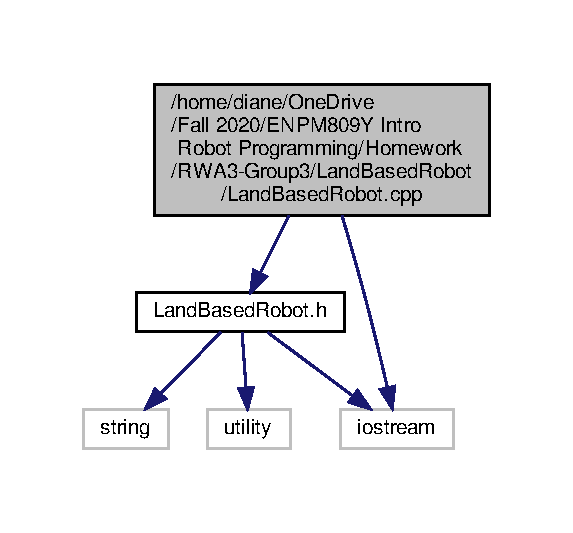
\includegraphics[width=275pt]{_land_based_robot_8cpp__incl}
\end{center}
\end{figure}
\subsection*{Namespaces}
\begin{DoxyCompactItemize}
\item 
 \hyperlink{namespacerwa3}{rwa3}
\end{DoxyCompactItemize}

\hypertarget{_land_based_robot_8h}{}\section{/home/diane/\+One\+Drive/\+Fall 2020/\+E\+N\+P\+M809Y Intro Robot Programming/\+Homework/\+R\+W\+A3-\/\+Group3/\+Land\+Based\+Robot/\+Land\+Based\+Robot.h File Reference}
\label{_land_based_robot_8h}\index{/home/diane/\+One\+Drive/\+Fall 2020/\+E\+N\+P\+M809\+Y Intro Robot Programming/\+Homework/\+R\+W\+A3-\/\+Group3/\+Land\+Based\+Robot/\+Land\+Based\+Robot.\+h@{/home/diane/\+One\+Drive/\+Fall 2020/\+E\+N\+P\+M809\+Y Intro Robot Programming/\+Homework/\+R\+W\+A3-\/\+Group3/\+Land\+Based\+Robot/\+Land\+Based\+Robot.\+h}}
{\ttfamily \#include $<$string$>$}\newline
{\ttfamily \#include $<$iostream$>$}\newline
{\ttfamily \#include $<$utility$>$}\newline
Include dependency graph for Land\+Based\+Robot.\+h\+:\nopagebreak
\begin{figure}[H]
\begin{center}
\leavevmode
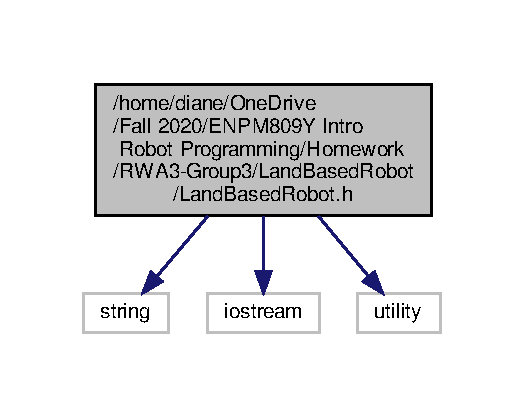
\includegraphics[width=252pt]{_land_based_robot_8h__incl}
\end{center}
\end{figure}
This graph shows which files directly or indirectly include this file\+:\nopagebreak
\begin{figure}[H]
\begin{center}
\leavevmode
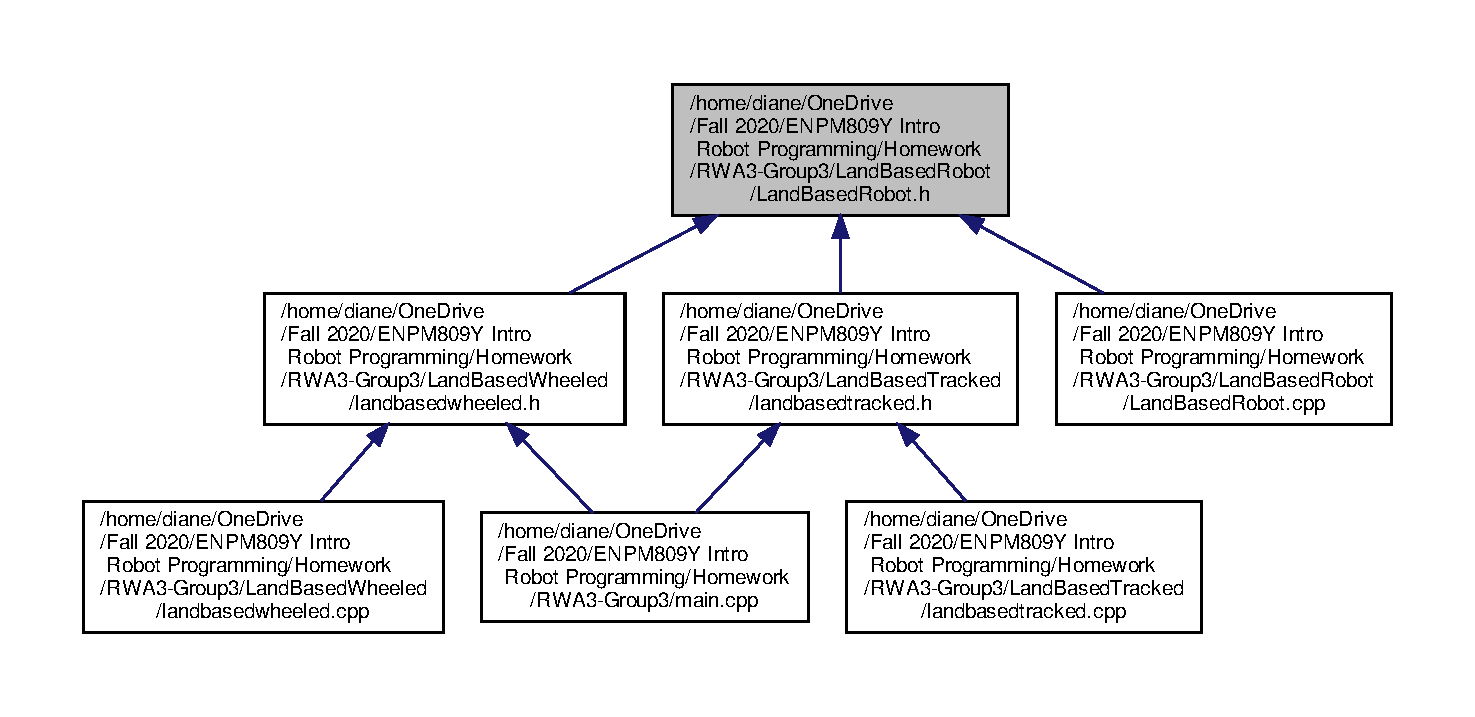
\includegraphics[width=350pt]{_land_based_robot_8h__dep__incl}
\end{center}
\end{figure}
\subsection*{Classes}
\begin{DoxyCompactItemize}
\item 
class \hyperlink{classrwa3_1_1_land_based_robot}{rwa3\+::\+Land\+Based\+Robot}
\end{DoxyCompactItemize}
\subsection*{Namespaces}
\begin{DoxyCompactItemize}
\item 
 \hyperlink{namespacerwa3}{rwa3}
\end{DoxyCompactItemize}

\hypertarget{landbasedtracked_8cpp}{}\section{/home/diane/\+One\+Drive/\+Fall 2020/\+E\+N\+P\+M809Y Intro Robot Programming/\+Homework/\+R\+W\+A3-\/\+Group3/\+Land\+Based\+Tracked/landbasedtracked.cpp File Reference}
\label{landbasedtracked_8cpp}\index{/home/diane/\+One\+Drive/\+Fall 2020/\+E\+N\+P\+M809\+Y Intro Robot Programming/\+Homework/\+R\+W\+A3-\/\+Group3/\+Land\+Based\+Tracked/landbasedtracked.\+cpp@{/home/diane/\+One\+Drive/\+Fall 2020/\+E\+N\+P\+M809\+Y Intro Robot Programming/\+Homework/\+R\+W\+A3-\/\+Group3/\+Land\+Based\+Tracked/landbasedtracked.\+cpp}}
{\ttfamily \#include \char`\"{}landbasedtracked.\+h\char`\"{}}\newline
{\ttfamily \#include $<$iostream$>$}\newline
Include dependency graph for landbasedtracked.\+cpp\+:\nopagebreak
\begin{figure}[H]
\begin{center}
\leavevmode
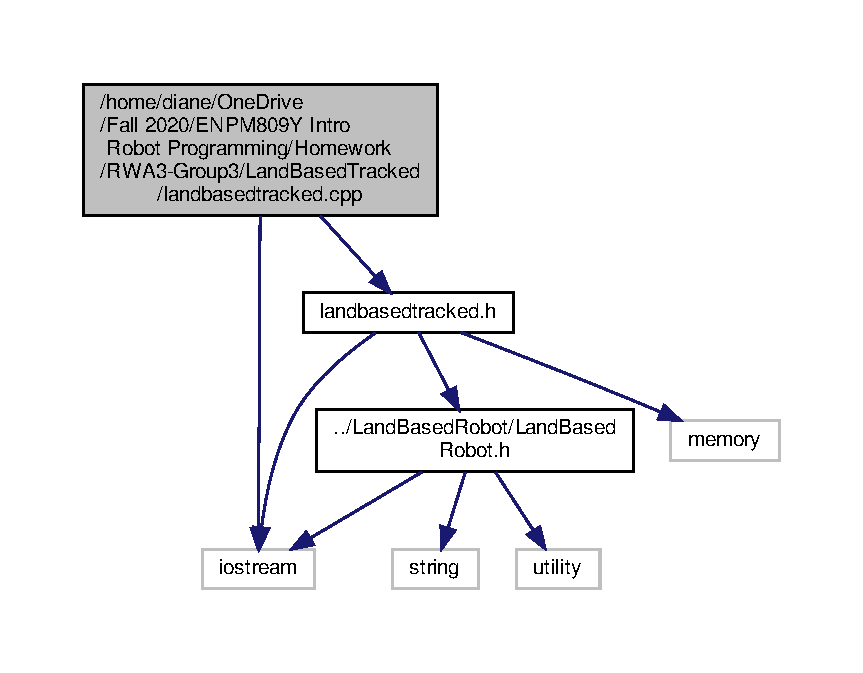
\includegraphics[width=350pt]{landbasedtracked_8cpp__incl}
\end{center}
\end{figure}

\hypertarget{landbasedtracked_8h}{}\section{/home/diane/\+One\+Drive/\+Fall 2020/\+E\+N\+P\+M809Y Intro Robot Programming/\+Homework/\+Final-\/\+Project-\/\+Group3/src/\+Land\+Based\+Tracked/landbasedtracked.h File Reference}
\label{landbasedtracked_8h}\index{/home/diane/\+One\+Drive/\+Fall 2020/\+E\+N\+P\+M809\+Y Intro Robot Programming/\+Homework/\+Final-\/\+Project-\/\+Group3/src/\+Land\+Based\+Tracked/landbasedtracked.\+h@{/home/diane/\+One\+Drive/\+Fall 2020/\+E\+N\+P\+M809\+Y Intro Robot Programming/\+Homework/\+Final-\/\+Project-\/\+Group3/src/\+Land\+Based\+Tracked/landbasedtracked.\+h}}
{\ttfamily \#include $<$iostream$>$}\newline
{\ttfamily \#include $<$memory$>$}\newline
{\ttfamily \#include $<$utility$>$}\newline
{\ttfamily \#include \char`\"{}../\+Land\+Based\+Robot/\+Land\+Based\+Robot.\+h\char`\"{}}\newline
Include dependency graph for landbasedtracked.\+h\+:\nopagebreak
\begin{figure}[H]
\begin{center}
\leavevmode
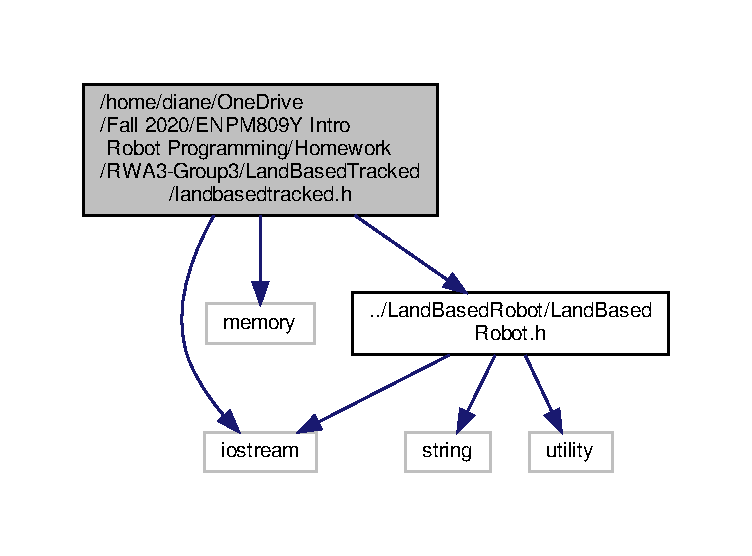
\includegraphics[width=350pt]{landbasedtracked_8h__incl}
\end{center}
\end{figure}
This graph shows which files directly or indirectly include this file\+:\nopagebreak
\begin{figure}[H]
\begin{center}
\leavevmode
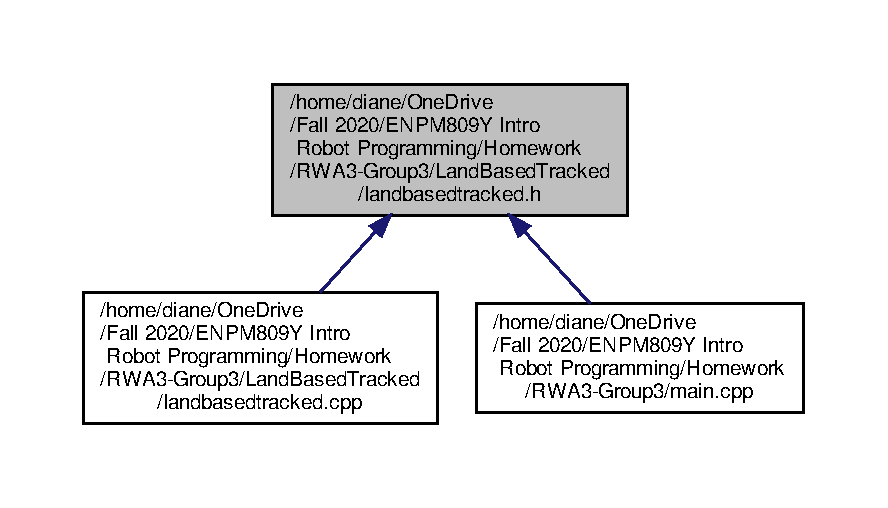
\includegraphics[width=350pt]{landbasedtracked_8h__dep__incl}
\end{center}
\end{figure}
\subsection*{Classes}
\begin{DoxyCompactItemize}
\item 
class \hyperlink{classfp_1_1_land_based_tracked}{fp\+::\+Land\+Based\+Tracked}
\end{DoxyCompactItemize}
\subsection*{Namespaces}
\begin{DoxyCompactItemize}
\item 
 \hyperlink{namespacefp}{fp}
\end{DoxyCompactItemize}

\hypertarget{landbasedwheeled_8cpp}{}\section{/home/diane/\+One\+Drive/\+Fall 2020/\+E\+N\+P\+M809Y Intro Robot Programming/\+Homework/\+R\+W\+A3-\/\+Group3/\+Land\+Based\+Wheeled/landbasedwheeled.cpp File Reference}
\label{landbasedwheeled_8cpp}\index{/home/diane/\+One\+Drive/\+Fall 2020/\+E\+N\+P\+M809\+Y Intro Robot Programming/\+Homework/\+R\+W\+A3-\/\+Group3/\+Land\+Based\+Wheeled/landbasedwheeled.\+cpp@{/home/diane/\+One\+Drive/\+Fall 2020/\+E\+N\+P\+M809\+Y Intro Robot Programming/\+Homework/\+R\+W\+A3-\/\+Group3/\+Land\+Based\+Wheeled/landbasedwheeled.\+cpp}}
{\ttfamily \#include \char`\"{}landbasedwheeled.\+h\char`\"{}}\newline
{\ttfamily \#include $<$iostream$>$}\newline
Include dependency graph for landbasedwheeled.\+cpp\+:\nopagebreak
\begin{figure}[H]
\begin{center}
\leavevmode
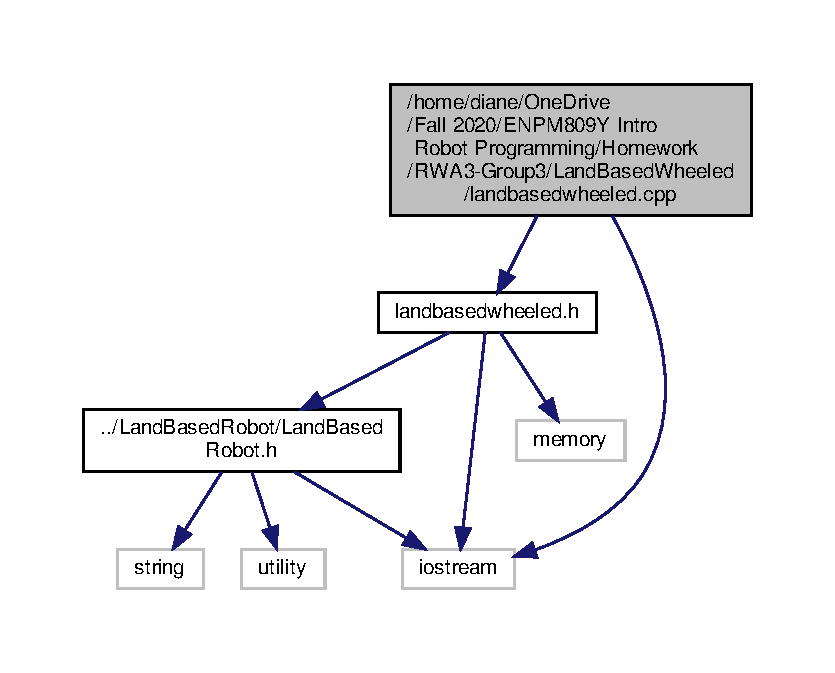
\includegraphics[width=350pt]{landbasedwheeled_8cpp__incl}
\end{center}
\end{figure}

\hypertarget{landbasedwheeled_8h}{}\section{/home/diane/\+One\+Drive/\+Fall 2020/\+E\+N\+P\+M809Y Intro Robot Programming/\+Homework/\+Final-\/\+Project-\/\+Group3/src/\+Land\+Based\+Wheeled/landbasedwheeled.h File Reference}
\label{landbasedwheeled_8h}\index{/home/diane/\+One\+Drive/\+Fall 2020/\+E\+N\+P\+M809\+Y Intro Robot Programming/\+Homework/\+Final-\/\+Project-\/\+Group3/src/\+Land\+Based\+Wheeled/landbasedwheeled.\+h@{/home/diane/\+One\+Drive/\+Fall 2020/\+E\+N\+P\+M809\+Y Intro Robot Programming/\+Homework/\+Final-\/\+Project-\/\+Group3/src/\+Land\+Based\+Wheeled/landbasedwheeled.\+h}}
{\ttfamily \#include \char`\"{}../\+Land\+Based\+Robot/\+Land\+Based\+Robot.\+h\char`\"{}}\newline
{\ttfamily \#include $<$iostream$>$}\newline
{\ttfamily \#include $<$memory$>$}\newline
{\ttfamily \#include $<$utility$>$}\newline
Include dependency graph for landbasedwheeled.\+h\+:\nopagebreak
\begin{figure}[H]
\begin{center}
\leavevmode
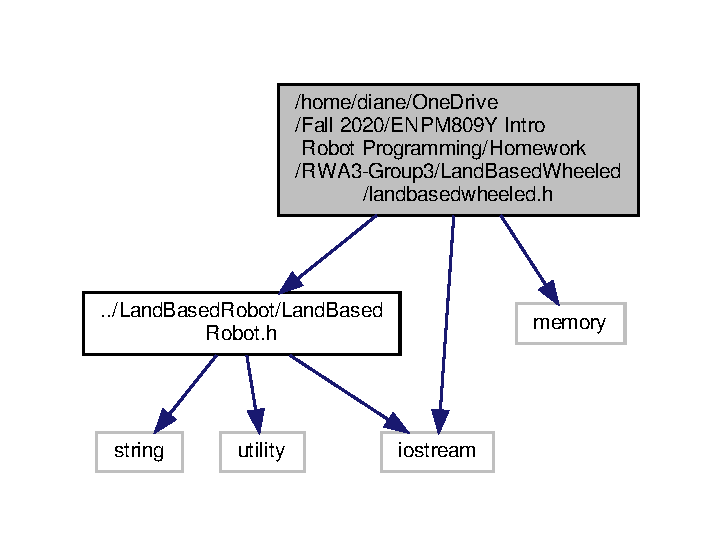
\includegraphics[width=350pt]{landbasedwheeled_8h__incl}
\end{center}
\end{figure}
This graph shows which files directly or indirectly include this file\+:\nopagebreak
\begin{figure}[H]
\begin{center}
\leavevmode
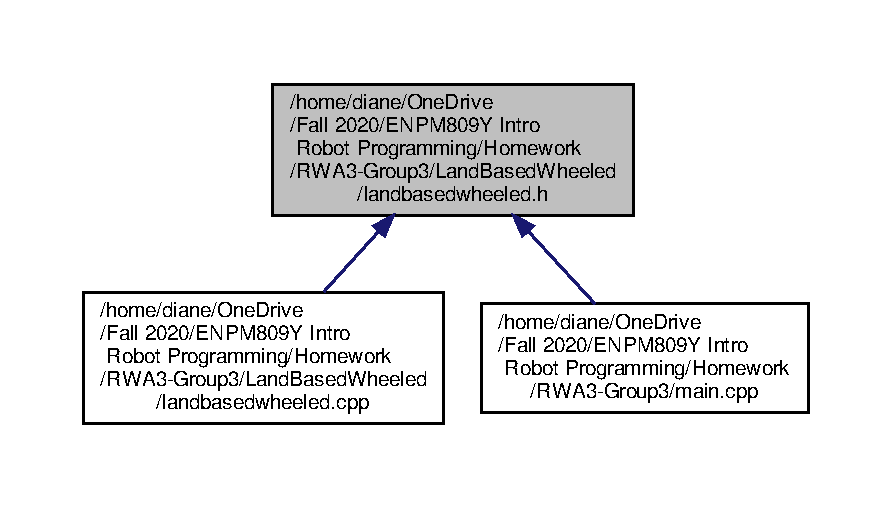
\includegraphics[width=350pt]{landbasedwheeled_8h__dep__incl}
\end{center}
\end{figure}
\subsection*{Classes}
\begin{DoxyCompactItemize}
\item 
class \hyperlink{classfp_1_1_land_based_wheeled}{fp\+::\+Land\+Based\+Wheeled}
\end{DoxyCompactItemize}
\subsection*{Namespaces}
\begin{DoxyCompactItemize}
\item 
 \hyperlink{namespacefp}{fp}
\end{DoxyCompactItemize}

\hypertarget{main_8cpp}{}\section{main.\+cpp File Reference}
\label{main_8cpp}\index{main.\+cpp@{main.\+cpp}}
{\ttfamily \#include $<$iostream$>$}\newline
Include dependency graph for main.\+cpp\+:\nopagebreak
\begin{figure}[H]
\begin{center}
\leavevmode
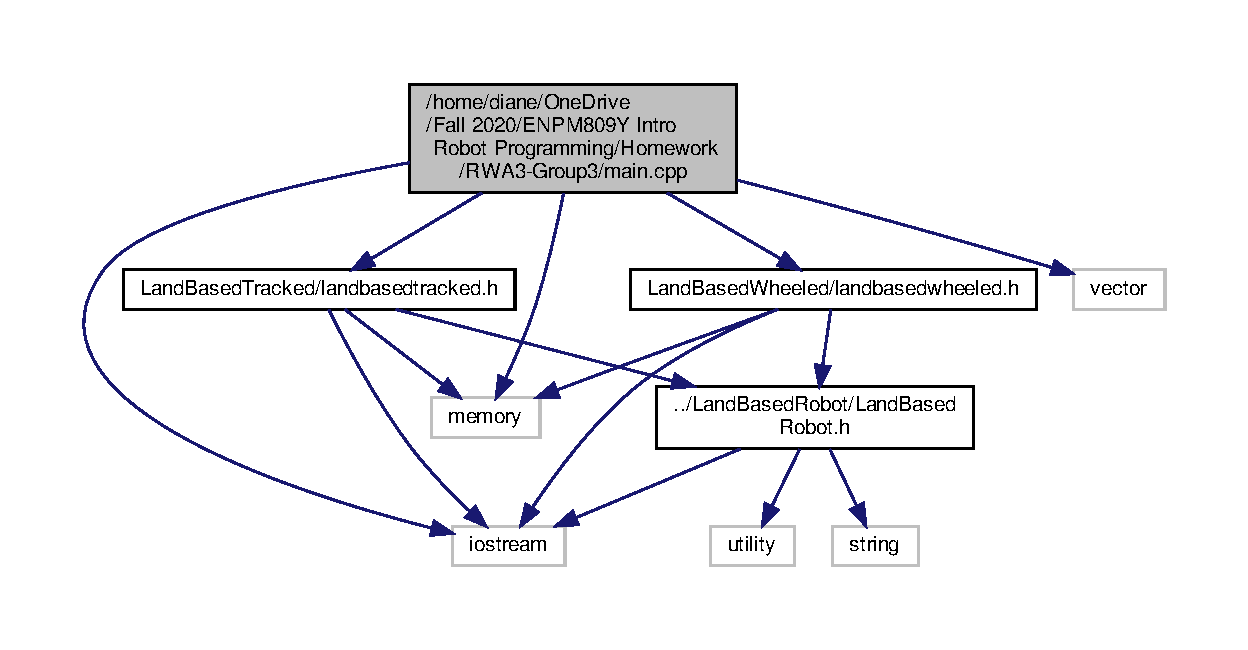
\includegraphics[width=136pt]{main_8cpp__incl}
\end{center}
\end{figure}
\subsection*{Macros}
\begin{DoxyCompactItemize}
\item 
\#define \hyperlink{main_8cpp_a3cfd3aa62338d12609f6d65bce97e9cd}{R\+O\+WS}~6
\begin{DoxyCompactList}\small\item\em Number of Rows for the Maze. \end{DoxyCompactList}\item 
\#define \hyperlink{main_8cpp_ab59ad2ee1a48b83c2eef1f019ed8cc48}{C\+O\+LS}~8
\begin{DoxyCompactList}\small\item\em Number of Columns for the Maze. \end{DoxyCompactList}\end{DoxyCompactItemize}
\subsection*{Functions}
\begin{DoxyCompactItemize}
\item 
bool \hyperlink{main_8cpp_acfa4bb7c74cebff4cd34982630e27e5a}{Check\+Wall} (char maze\mbox{[}6\mbox{]}\mbox{[}8\mbox{]}, int \&x, int \&y)
\item 
bool \hyperlink{main_8cpp_a15ab7ba904c0f46588d62b302075a8c3}{Check\+Outside} (int \&x, int \&y)
\item 
bool \hyperlink{main_8cpp_aefd146022809df49fb9ba712ecb00ffe}{Back\+Track} (char maze\mbox{[}6\mbox{]}\mbox{[}8\mbox{]}, int \&x, int \&y)
\item 
void \hyperlink{main_8cpp_a41b5491830aa7fa26ded753af127966f}{display\+\_\+maze} (char maze\mbox{[}6\mbox{]}\mbox{[}8\mbox{]})
\item 
bool \hyperlink{main_8cpp_acafe6eccc9f6c953bc9b609f732b2273}{Find\+Path} (char maze\mbox{[}6\mbox{]}\mbox{[}8\mbox{]}, int x, int y)
\item 
int \hyperlink{main_8cpp_ae66f6b31b5ad750f1fe042a706a4e3d4}{main} ()
\end{DoxyCompactItemize}


\subsection{Macro Definition Documentation}
\mbox{\Hypertarget{main_8cpp_ab59ad2ee1a48b83c2eef1f019ed8cc48}\label{main_8cpp_ab59ad2ee1a48b83c2eef1f019ed8cc48}} 
\index{main.\+cpp@{main.\+cpp}!C\+O\+LS@{C\+O\+LS}}
\index{C\+O\+LS@{C\+O\+LS}!main.\+cpp@{main.\+cpp}}
\subsubsection{\texorpdfstring{C\+O\+LS}{COLS}}
{\footnotesize\ttfamily \#define C\+O\+LS~8}



Number of Columns for the Maze. 

\mbox{\Hypertarget{main_8cpp_a3cfd3aa62338d12609f6d65bce97e9cd}\label{main_8cpp_a3cfd3aa62338d12609f6d65bce97e9cd}} 
\index{main.\+cpp@{main.\+cpp}!R\+O\+WS@{R\+O\+WS}}
\index{R\+O\+WS@{R\+O\+WS}!main.\+cpp@{main.\+cpp}}
\subsubsection{\texorpdfstring{R\+O\+WS}{ROWS}}
{\footnotesize\ttfamily \#define R\+O\+WS~6}



Number of Rows for the Maze. 



\subsection{Function Documentation}
\mbox{\Hypertarget{main_8cpp_aefd146022809df49fb9ba712ecb00ffe}\label{main_8cpp_aefd146022809df49fb9ba712ecb00ffe}} 
\index{main.\+cpp@{main.\+cpp}!Back\+Track@{Back\+Track}}
\index{Back\+Track@{Back\+Track}!main.\+cpp@{main.\+cpp}}
\subsubsection{\texorpdfstring{Back\+Track()}{BackTrack()}}
{\footnotesize\ttfamily bool Back\+Track (\begin{DoxyParamCaption}\item[{char}]{maze\mbox{[}6\mbox{]}\mbox{[}8\mbox{]},  }\item[{int \&}]{x,  }\item[{int \&}]{y }\end{DoxyParamCaption})}

Function to backtrack if the coordinate has been visited and there is no path found 
\begin{DoxyParams}{Parameters}
{\em maze} & the 2D array of character for the maze \\
\hline
{\em x} & integer of the x coordinate \\
\hline
{\em y} & integer of the y coordinate \\
\hline
\end{DoxyParams}
\begin{DoxyReturn}{Returns}

\end{DoxyReturn}
\mbox{\Hypertarget{main_8cpp_a15ab7ba904c0f46588d62b302075a8c3}\label{main_8cpp_a15ab7ba904c0f46588d62b302075a8c3}} 
\index{main.\+cpp@{main.\+cpp}!Check\+Outside@{Check\+Outside}}
\index{Check\+Outside@{Check\+Outside}!main.\+cpp@{main.\+cpp}}
\subsubsection{\texorpdfstring{Check\+Outside()}{CheckOutside()}}
{\footnotesize\ttfamily bool Check\+Outside (\begin{DoxyParamCaption}\item[{int \&}]{x,  }\item[{int \&}]{y }\end{DoxyParamCaption})}

Check\+Outside Function\+: Function to check if the desired direction is outside of the maze 
\begin{DoxyParams}{Parameters}
{\em maze} & the 2D array of character for the maze \\
\hline
{\em x} & integer of the x coordinate \\
\hline
{\em y} & integer of the y coordinate \\
\hline
\end{DoxyParams}
\begin{DoxyReturn}{Returns}

\end{DoxyReturn}
\mbox{\Hypertarget{main_8cpp_acfa4bb7c74cebff4cd34982630e27e5a}\label{main_8cpp_acfa4bb7c74cebff4cd34982630e27e5a}} 
\index{main.\+cpp@{main.\+cpp}!Check\+Wall@{Check\+Wall}}
\index{Check\+Wall@{Check\+Wall}!main.\+cpp@{main.\+cpp}}
\subsubsection{\texorpdfstring{Check\+Wall()}{CheckWall()}}
{\footnotesize\ttfamily bool Check\+Wall (\begin{DoxyParamCaption}\item[{char}]{maze\mbox{[}6\mbox{]}\mbox{[}8\mbox{]},  }\item[{int \&}]{x,  }\item[{int \&}]{y }\end{DoxyParamCaption})}

Check\+Wall Function\+: Function to check if there is a wall in the desired direction 
\begin{DoxyParams}{Parameters}
{\em maze} & the 2D array of character for the maze \\
\hline
{\em x} & integer of the x coordinate \\
\hline
{\em y} & integer of the y coordinate \\
\hline
\end{DoxyParams}
\begin{DoxyReturn}{Returns}

\end{DoxyReturn}
\mbox{\Hypertarget{main_8cpp_a41b5491830aa7fa26ded753af127966f}\label{main_8cpp_a41b5491830aa7fa26ded753af127966f}} 
\index{main.\+cpp@{main.\+cpp}!display\+\_\+maze@{display\+\_\+maze}}
\index{display\+\_\+maze@{display\+\_\+maze}!main.\+cpp@{main.\+cpp}}
\subsubsection{\texorpdfstring{display\+\_\+maze()}{display\_maze()}}
{\footnotesize\ttfamily void display\+\_\+maze (\begin{DoxyParamCaption}\item[{char}]{maze\mbox{[}6\mbox{]}\mbox{[}8\mbox{]} }\end{DoxyParamCaption})}

Function to display the maze 
\begin{DoxyParams}{Parameters}
{\em maze} & the 2d array of characters for the maze \\
\hline
\end{DoxyParams}
\mbox{\Hypertarget{main_8cpp_acafe6eccc9f6c953bc9b609f732b2273}\label{main_8cpp_acafe6eccc9f6c953bc9b609f732b2273}} 
\index{main.\+cpp@{main.\+cpp}!Find\+Path@{Find\+Path}}
\index{Find\+Path@{Find\+Path}!main.\+cpp@{main.\+cpp}}
\subsubsection{\texorpdfstring{Find\+Path()}{FindPath()}}
{\footnotesize\ttfamily bool Find\+Path (\begin{DoxyParamCaption}\item[{char}]{maze\mbox{[}6\mbox{]}\mbox{[}8\mbox{]},  }\item[{int}]{x,  }\item[{int}]{y }\end{DoxyParamCaption})}

Find\+Path Function is a recursive function to iterate through the maze by checking North, East, South, and West. It checks if there is a wall at the position or if its outside of the maze, then proceeds by placing a + sign at the position and updates. 
\begin{DoxyParams}{Parameters}
{\em maze} & the 2D array of character for the maze \\
\hline
{\em x} & integer of the x coordinate \\
\hline
{\em y} & integer of the y coordinate \\
\hline
\end{DoxyParams}
\begin{DoxyReturn}{Returns}

\end{DoxyReturn}
If the x, y is at the goal position

If the coordinates is not at the goal position

Declare outside variable

Declare wall variable

Declare backtrack variable

If x, y is outside of the maze or is a wall

Mark path

Checking North

Checking East

Checking South

Checking West

Backtrack by setting the coordinate back to . \mbox{\Hypertarget{main_8cpp_ae66f6b31b5ad750f1fe042a706a4e3d4}\label{main_8cpp_ae66f6b31b5ad750f1fe042a706a4e3d4}} 
\index{main.\+cpp@{main.\+cpp}!main@{main}}
\index{main@{main}!main.\+cpp@{main.\+cpp}}
\subsubsection{\texorpdfstring{main()}{main()}}
{\footnotesize\ttfamily int main (\begin{DoxyParamCaption}{ }\end{DoxyParamCaption})}

Maze array is reversed to print it out with respect to the coordinate system

Initialize the variables for the starting position

Initialize temporary variables s\+\_\+x and s\+\_\+y to save the new input

User Input

While Loop to determine if start and goal position are inside of the maze and not a wall

This if loop checks if the desired starting position is outside of the maze.

set the s array to coordinates x, y

Initialize temporary variables g\+\_\+x and g\+\_\+y to save the new input

This if loop checks if the desired goal position is outside of the maze.

set the g array to coordinates x, y 
%--- End generated contents ---

% Index
\backmatter
\newpage
\phantomsection
\clearemptydoublepage
\addcontentsline{toc}{chapter}{Index}
\printindex

\end{document}
